% Compile with XeLaTeX or LuaLaTeX
\documentclass[10pt]{article}  % Spivak uses ~10pt

% -----------------------------
% Fonts
% -----------------------------
\usepackage{fontspec}
\setmainfont{TeX Gyre Pagella}
\usepackage{unicode-math}
\setmathfont{Libertinus Math}

% -----------------------------
% Page layout
% -----------------------------
\usepackage[margin=2.5cm]{geometry}
\usepackage[parfill]{parskip}

% -----------------------------
% Theorems and QED
% -----------------------------
\usepackage{amsthm}
\usepackage{tcolorbox}
\tcbuselibrary{breakable}

% QED symbol like Spivak (tall gray rectangle)
\renewcommand{\qedsymbol}{\textcolor{black}{\rule{1ex}{2.2ex}}}

\newtheorem{theorem}{Theorem}
\newtheorem{axiom}{Axiom}
\newtheorem{definition}{Definition}

% -----------------------------
% Misc packages
% -----------------------------
\usepackage{graphicx, subfig}
\usepackage{booktabs, array}
\usepackage{paralist, verbatim}
\usepackage{xcolor, pagecolor}
\usepackage{fancyhdr}
\pagestyle{fancy}
\renewcommand{\headrulewidth}{0pt}
\lhead{}\chead{}\rhead{}
\lfoot{}\cfoot{\thepage}\rfoot{}
\usepackage{sectsty}
\allsectionsfont{\sffamily\mdseries\upshape}
\usepackage[nottoc,notlof,notlot]{tocbibind}
\usepackage[titles,subfigure]{tocloft}
\renewcommand{\cftsecfont}{\rmfamily\mdseries\upshape}
\renewcommand{\cftsecpagefont}{\rmfamily\mdseries\upshape}
\usepackage{changepage, comment}
% Define a light gray
\definecolor{lightgraypaper}{RGB}{240,240,240}
% Set the page background
\pagecolor{lightgraypaper}
\color{black} % keep text black

\title{Calculus by Elliott Mendelson}
\author{Noah Lewis}
\begin{document}
\maketitle

\tableofcontents

% ===============================
% 30-Week Calc 1 & Calc 2 Review Schedule
% ===============================

\section{Functions}
\begin{tcolorbox}[title=Problem 1, breakable]
    Show that in a ring, $0a = a0 = 0$.
\end{tcolorbox}

\begin{proof}
    Let $R$ be a ring and $a$ be an arbitrary element in $R$.
    Then
    \begin{align*}
        0a &= 0a + 0 &&\text{Rule 3} \\
            &= 0a + (0a + (-0a)) &&\text{Rule 4} \\
            &= (0a + 0a) + (-0a) &&\text{Rule 2} \\
            &= ((0 + 0)a) + (-0a) &&\text{Rule 6} \\
            &= 0a + (-0a) &&\text{Rule 3} \\
            &= 0 &&\text{Rule 3}
    \end{align*}
    Similarly 
    \begin{align*}
        a0 &= a0 + 0 &&\text{Rule 3} \\
            &= a0 + (a0 + (-a0)) &&\text{Rule 4} \\
            &= (a0 + a0) + (-a0) &&\text{Rule 2} \\
            &= (a(0 + 0)) + (-a0) &&\text{Rule 6} \\
            &= a0 + (-a0) &&\text{Rule 3} \\
            &= 0 &&\text{Rule 3}
    \end{align*}
    Thus $a0 = 0a = 0$.
\end{proof}

\begin{tcolorbox}[title=Problem 2, breakable]
    Prove part d of Theorem 6.1:
    Show that in a ring the additive identity is unique,
        by supposing $0$ and $0'$ satisfy Rule 3
        and proving that $0 = 0'$.
\end{tcolorbox}

\begin{proof}
    Let $R$ be a ring and suppose there exists $0 \in R$
        and $0' \in R$ such that 
        for all $a \in R$, $a + 0 = a$ and $a + 0' = a$.
    Then $a + 0 = a = a + 0'$.
    By Additive Cancellation $0 = 0'$.
\end{proof}

\begin{tcolorbox}[title=Problem 3, breakable]
    Show that in a ring $(-a)b = a(-b) = -(ab)$.
\end{tcolorbox}

\begin{proof}
    Let $R$ be a ring and $a, b \in R$. Then
    \begin{align*}
        0 = (a + (-a))b 
        \iff &0 = ab + (-a)b &&\text{Rule 6} \\
        \iff &-(ab) + 0 = -(ab) + (ab + (-a)b) \\
        \iff &-(ab) = -(ab) + (ab + (-a)b) &&\text{Rule 3} \\
        \iff &-(ab) = (-(ab) + ab) + (-a)b &&\text{Rule 2} \\
        \iff &-(ab) = 0 + (-a)b &&\text{Rule 4} \\
        \iff &-(ab) = (-a)b + 0 &&\text{Rule 1} \\
        \iff &-(ab) = (-a)b &&\text{Rule 3}
    \end{align*}
    Also
    \begin{align*}
        0 = a(b + (-b)) 
        \iff &0 = ab + a(-b) &&\text{Rule 6} \\
        \iff &-(ab) + 0 = -(ab) + ((ab) + a(-b))  \\
        \iff &-(ab) = -(ab) + ((ab) + a(-b)) &&\text{Rule 3} \\
        \iff &-(ab) = (-(ab) + (ab)) + a(-b) &&\text{Rule 2} \\
        \iff &-(ab) = 0 + a(-b) &&\text{Rule 4} \\
        \iff &-(ab) = a(-b) + 0 &&\text{Rule 1} \\
        \iff &-(ab) = a(-b) &&\text{Rule 3}
    \end{align*}
    Thus $(-a)b = a(-b) = -(ab)$.
\end{proof}

\begin{tcolorbox}[title=Problem 4, breakable]
    Show that in a ring $(-a)(-b) = ab$.
\end{tcolorbox}

\begin{proof}
    \begin{align*}
        (-a)(-b) + -(ab) &= a(-(-b)) + a(-b) && \text{Rule 6} \\
                        &= a((-(-b)) + (-b)) && \text{Rule 2} \\
                        &= a \cdot 0 && \text{Rule 4} \\
                        &= 0 && \text{Rule 3}
    \end{align*}
    Thus $(-a)(-b) = ab$.
\end{proof}

\begin{tcolorbox}[title=Problem 5, breakable]
    Prove the following facts about subtraction in a ring $R$,
    where $a, b, c \in R$.

    (a) $a - a = 0$.

    (b) $a(b - c) = ab - ac$.

    (c) $(b - c)a = ba - ca$.
\end{tcolorbox}

\begin{proof}
    Let $R$ be a ring and $a, b, c \in R$.
    Then $a - a = a + (-a) = 0$ Rule 4.
    Also, $a(b - c) = a(b + (-c)) = ab + a(-c)$ Rule 6.
    Then, $ab + a(-c) = ab + -(ac) \text{ Problem 3 } = ab - ac$.
    Similarly, $(b - c)a = (b + (-c))a = ba + (-c)a$ Rule 6.
    Then, $ba + (-c)a = ba + -(ca) \text{ Problem 3 } = ba - ca$.
\end{proof}

\begin{tcolorbox}[title=Problem 8, breakable]
    We generalize Exercises 6 and 7: Let $R$
    be any commutative ring (other than the zero ring).
    Define $M_2(R)$ as the set of $2 \times 2$
    matrices with entries from $R$. Show that $M_2(R)$
    is a ring which is not commutative. (Note that 
    for the most part the proofs in Exercises 6 and 
    7 life over without change.)
\end{tcolorbox}

\begin{proof}
    Let $R$ be a ring and 
    \[a, b, c, e, f, g, h, i, j, k, l \in R\]
    We first show associativity with respect to $+$.
    \[\begin{bmatrix}
        a & b \\
        c & d
    \end{bmatrix} \in M_2(R) \text{, }
    \begin{bmatrix}
        c & f \\
        g & h
    \end{bmatrix} \in M_2(R) \text{ and }
    \begin{bmatrix}
        i & j \\
        k & l
    \end{bmatrix} \in M_2(R)\]
    Then 
    \[\begin{bmatrix}
        a & b \\
        c & d
    \end{bmatrix} + \begin{bmatrix}
        c & f \\
        g & h
    \end{bmatrix} = \begin{bmatrix}
        a+c & b+f \\
        c+g & d+h
    \end{bmatrix} = \begin{bmatrix}
        c+a & f+b \\
        g+c & h+d
    \end{bmatrix} = \begin{bmatrix}
        c & f \\
        g & h
    \end{bmatrix} + \begin{bmatrix}
        a & b \\
        c & d
    \end{bmatrix}\]
    We now show associativity with respect to $+$.
\[\left(\begin{bmatrix}
        a & b \\
        c & d
    \end{bmatrix} + \begin{bmatrix}
        c & f \\
        g & h
    \end{bmatrix}\right) + \begin{bmatrix}
        i & j \\
        k & l
    \end{bmatrix} = \begin{bmatrix}
        a+c & b+f \\
        c+g & d+h
    \end{bmatrix} +\begin{bmatrix}
        i & j \\
        k & l
    \end{bmatrix} = \begin{bmatrix}
        (a+c)+i & (b+f)+j \\
        (c+g)+k & (d+h)+l
    \end{bmatrix}\] \[= \begin{bmatrix}
        a+(c+i) & b+(f+j) \\
        c+(g+k) & d+(h+l)
    \end{bmatrix} = \begin{bmatrix}
        a & b \\
        c & d
    \end{bmatrix} + \begin{bmatrix}
        c+i & f+j \\
        g+k & h+l
    \end{bmatrix} = \begin{bmatrix}
        a & b \\
        c & d
    \end{bmatrix} + \left(\begin{bmatrix}
        c & f \\
        g & h
    \end{bmatrix} + \begin{bmatrix}
        i & j \\
        k & l
    \end{bmatrix}\right)\]
    We now show the existence of an additive inverse.
    \[\begin{bmatrix}
        a & b \\
        c & d
    \end{bmatrix} -\begin{bmatrix}
        a & b \\
        c & d
    \end{bmatrix} = \begin{bmatrix}
        a-a & b-b \\
        c-c & d-d
    \end{bmatrix} = \begin{bmatrix}
        0 & 0 \\
        0 & 0
    \end{bmatrix}\]
    We now show the existence of the additive identity.
    \[\begin{bmatrix}
        a & b \\
        c & d
    \end{bmatrix} + \begin{bmatrix}
        0 & 0 \\
        0 & 0
    \end{bmatrix} = \begin{bmatrix}
        a+0 & b+0 \\
        c+0 & d+0
    \end{bmatrix} = \begin{bmatrix}
        a & b \\
        c & d
    \end{bmatrix}\]
    We now show left distributivity.
    \[
    \begin{bmatrix}
        a & b \\
        c & d
    \end{bmatrix}
    \left(
    \begin{bmatrix}
        e & f \\
        g & h
    \end{bmatrix}
    +
    \begin{bmatrix}
        i & j \\
        k & l
    \end{bmatrix}
    \right)
    =
    \begin{bmatrix}
        a & b \\
        c & d
    \end{bmatrix}
    \begin{bmatrix}
        e+i & f+j \\
        g+k & h+l
    \end{bmatrix}
    =
    \begin{bmatrix}
        a(e+i) + b(g+k) & a(f+j) + b(h+l) \\
        c(e+i) + d(g+k) & c(f+j) + d(h+l)
    \end{bmatrix}
    \]
    \[
    =
    \begin{bmatrix}
        ae + bg & af + bh \\
        ce + dg & cf + dh
    \end{bmatrix}
    +
    \begin{bmatrix}
        ai + bk & aj + bl \\
        ci + dk & cj + dl
    \end{bmatrix}
    =
    \begin{bmatrix}
        a & b \\
        c & d
    \end{bmatrix}
    \begin{bmatrix}
        e & f \\
        g & h
    \end{bmatrix}
    +
    \begin{bmatrix}
        a & b \\
        c & d
    \end{bmatrix}
    \begin{bmatrix}
        i & j \\
        k & l
    \end{bmatrix}.
    \]
    We now show right distributivity.
    \[
    \left(
    \begin{bmatrix}
        e & f \\
        g & h
    \end{bmatrix}
    +
    \begin{bmatrix}
        i & j \\
        k & l
    \end{bmatrix}
    \right)
    \begin{bmatrix}
        a & b \\
        c & d
    \end{bmatrix}
    =
    \begin{bmatrix}
        e+i & f+j \\
        g+k & h+l
    \end{bmatrix}
    \begin{bmatrix}
        a & b \\
        c & d
    \end{bmatrix}
    =
    \begin{bmatrix}
        (e+i)a + (f+j)c & (e+i)b + (f+j)d \\
        (g+k)a + (h+l)c & (g+k)b + (h+l)d
    \end{bmatrix}
    \]
    \[
    =
    \begin{bmatrix}
        ea + fc & eb + fd \\
        ga + hc & gb + hd
    \end{bmatrix}
    +
    \begin{bmatrix}
        ia + jc & ib + jd \\
        ka + lc & kb + ld
    \end{bmatrix}
    =
    \begin{bmatrix}
        e & f \\
        g & h
    \end{bmatrix}
    \begin{bmatrix}
        a & b \\
        c & d
    \end{bmatrix}
    +
    \begin{bmatrix}
        i & j \\
        k & l
    \end{bmatrix}
    \begin{bmatrix}
        a & b \\
        c & d
    \end{bmatrix}
    \]
    We now show matrix multiplication is not commutative 
        by giving a counterexample.
    Consider
    \[
    \begin{bmatrix}
    1 & 2 \\
    0 & 1
    \end{bmatrix}
    \begin{bmatrix}
    1 & 0 \\
    3 & 1
    \end{bmatrix}
    =
    \begin{bmatrix}
    1+6 & 2 \\
    3 & 1
    \end{bmatrix}
    =
    \begin{bmatrix}
    7 & 2 \\
    3 & 1
    \end{bmatrix}
    \]
    But multiplying the same matrices in the opposite order gives
    \[
    \begin{bmatrix}
    1 & 0 \\
    3 & 1
    \end{bmatrix}
    \begin{bmatrix}
    1 & 2 \\
    0 & 1
    \end{bmatrix}
    =
    \begin{bmatrix}
    1 & 2 \\
    3 & 7
    \end{bmatrix}.
    \]
    Since
    \[
    \begin{bmatrix}
    7 & 2 \\
    3 & 1
    \end{bmatrix}
    \neq
    \begin{bmatrix}
    1 & 2 \\
    3 & 7
    \end{bmatrix}
    \]
    matrix multiplication is not commutative.
\end{proof}

Let $R = \{0, a, \ldots\}$ such that $0 \ne a$.
\[
A = \begin{bmatrix} 0 & a \\ 0 & 0 \end{bmatrix}, \quad
B = \begin{bmatrix} 0 & 0 \\ a & 0 \end{bmatrix}
\]
\[
AB = \begin{bmatrix} a^2 & 0 \\ 0 & 0 \end{bmatrix} \neq 
BA = \begin{bmatrix} 0 & 0 \\ 0 & a^2 \end{bmatrix}
\]

\begin{tcolorbox}[title=Problem 9, breakable]
    Check that Example 6.14 is indeed a ring; that is,
    let $C[0, 1]$ be a set of functions defined from the closed 
    unit interval $[0, 1]$ to the real numbers that 
    are continuous. Define the sum and product of two 
    functions point-wise: $(f + g)(x) = f(x) + g(x)$
    and $(fg)(x) = f(x)g(x)$. Show that $C[0, 1]$ is a 
    commutative ring. (You may use theorems from calculus).
\end{tcolorbox}

\begin{proof}
    Let $x \in [0, 1]$ and $f, g, l : [0, 1] \longrightarrow \mathbb{R}$.
    Since $f(x), g(x), l(x) \in \mathbb{R}$ and $\mathbb{R}$ is a ring, standard ring operations (associativity, distributivity, etc.) hold.
    We first show commutativity over addition
    \[
    (f + g)(x) = f(x) + g(x) = g(x) + f(x) = (g + f)(x)
    \]
    Next, associativity over addition
    \[
    ((f + g) + l)(x) = (f + g)(x) + l(x) = f(x) + g(x) + l(x) = f(x) + (g + l)(x) = (f + (g + l))(x).
    \]
    Existence of additive inverses
    \[
    (f + (-f))(x) = f(x) + (-f(x)) = 0
    \]
    Additive identity
    \[
    (f + 0)(x) = f(x) + 0(x) = f(x)
    \]
    Commutativity of multiplication
    \[
    (fg)(x) = f(x) g(x) = g(x) f(x) = (gf)(x)
    \]
    Associativity of multiplication
    \[
    ((fg)l)(x) = (fg)(x) l(x) = f(x) g(x) l(x) = f(x) (gl)(x) = (f(gl))(x)
    \]
    Distributivity from the left
    \[
    f(g + l)(x) = f(x)(g + l)(x) = f(x)(g(x) + l(x)) = f(x)g(x) + f(x)l(x) = (fg + fl)(x)
    \]
    Distributivity from the right
    \[
    (f + g)l(x) = (f + g)(x) \, l(x) = (f(x) + g(x))l(x) = f(x)l(x) + g(x)l(x) = (fl + gl)(x)
    \]
\end{proof}

\begin{tcolorbox}[title=Problem 11, breakable]
    Let $\mathbb{C}$ be the complex numbers. That inverse
    \[\mathbb{C} = \{a + bi \mid a, b, \in \mathbb{R}\}\]
    where $i$ is the square root of $-1$ (that is, $i \cdot i = 1$).
    Here 
    \[(a + bi) + (c + di) = (a + c) + (bi + di)\]
    and 
    \[(a + bi)(c + di) = (ac - bd) + (ad + bc)i\]
    Show that $\mathbb{C}$ is a commutative ring.
\end{tcolorbox}

\begin{proof}
    Let $a + bi, c + di, e + fi \in \mathbb{C}$.
    We first show commutativity over addition
    \[
    (a + bi) + (c + di) = (a + c) + (bi + di) = (c + a) + (di + bi) = (c + di) + (a + bi)
    \]
    Next, associativity over addition
    \[
    ((f + g) + l)(x) = (f + g)(x) + l(x) = f(x) + g(x) + l(x) = f(x) + (g + l)(x) = (f + (g + l))(x).
    \]
    Existence of additive inverses
    \[
    (f + (-f))(x) = f(x) + (-f(x)) = 0
    \]
    Additive identity
    \[
    (f + 0)(x) = f(x) + 0(x) = f(x)
    \]
    Commutativity of multiplication
    \[
    (fg)(x) = f(x) g(x) = g(x) f(x) = (gf)(x)
    \]
    Associativity of multiplication
    \[
    ((fg)l)(x) = (fg)(x) l(x) = f(x) g(x) l(x) = f(x) (gl)(x) = (f(gl))(x)
    \]
    Distributivity from the left
    \[
    f(g + l)(x) = f(x)(g + l)(x) = f(x)(g(x) + l(x)) = f(x)g(x) + f(x)l(x) = (fg + fl)(x)
    \]
    Distributivity from the right
    \[
    (f + g)l(x) = (f + g)(x) \, l(x) = (f(x) + g(x))l(x) = f(x)l(x) + g(x)l(x) = (fl + gl)(x)
    \]
\end{proof}

\begin{tcolorbox}[title=Problem 15, breakable]
    Verify that 6.10 is a ring.
    Namely, let $R$ and $S$ be arbitrary rings.
    Define addition and subtraction appropriately
        to make $R \times S$ a ring,
        where $R \times S$ is the set of ordered pairs
        with the first entry from $R$ and second entry 
        from $S$. 
    Now generalize this to the set $R_1 \times R_2 \times \cdots R_n$
    of $n$-tuples with entries from the rings $R_i$.
    This new ring is called the \textbf{direct product}
    of the rings $R_i$.
\end{tcolorbox}
% Week 1: Review domain, range, composition, and inverse functions. Make sure you understand function behavior and graphs.

\section{Limits}
\subsection{Area of a Disc of Radius $r$}

\begin{tcolorbox}[title=Problem 3, breakable]
    (a) Suppose that the sides of a rectangles $S$ have lengths 
        $r$ and $s$. What are the lengths of the sides  of the 
        rectangle $F_{a, b}(S)$, i.e. of the rectangle obtained 
        by the mixed dilation $F_{a, b}$?

    (b) What is the area of $F_{a, b}$?

    (c) If $S$ is a bounded region in the plane with area $A$,
        what is the area of $F_{a, b}(S)$?
\end{tcolorbox}

\textbf{Solution (a):}
\[F_{a, b}(S) \text{ has } ar \text{ width and } bs \text{ height.}\]
\textbf{Solution (b):}
\[\text{area}= ar \cdot bs = ab(rs)\]
\textbf{Solution (c):}
\[F_{a, b}(S) = ab(A)\]

\begin{tcolorbox}[title=Problem 4, breakable]
    (a) Show that the set of points $(u, v)$ satisfying the equation
        \[\left(\frac{u}{a}\right)^2 + \left(\frac{v}{b}\right)^2 = 1\]
        is the image of the circle of radius $1$ centered at $O$ under 
        the map $F_{a, b}$.

    (b) Let $a = 3$ and $b = 2$. Sketch this set, which is called an 
        \textbf{ellipse}.

    (c) Can you guess and motivate your guess as to what the area of the 
        region bounded by the ellipse in $(a)$ should be.
\end{tcolorbox}

\begin{proof}
    Let $C$ be the set of points making up the circle with radius $r = 1$ and center $O$.
    Let $P$ be an arbitrary point in $C$. Since $r = 1$, $d(O, P) = 1$.
    Let $L_1$ and $L_2$ be the vertical and horizontal lines through $O$, respectively.
    Drop perpendiculars from $P$ to $L_1$ and $L_2$, 
        and let $Q$ and $R$ be the feet of these perpendiculars on $L_1$ and $L_2$, respectively.
    Then $\triangle OQR$ is a right triangle with hypotenuse $\overline{OP}$, 
        and legs $\overline{OQ}$ and $\overline{OR}$ lying along $L_1$ and $L_2$.
    Let $u = d(OQ), v = d(OR)$ and by Pythagoras' Theorem $u^2 + v^2 = 1$.
    By applying the mapping $F_{a, b}$ to $\overline{OQ}, \overline{OR}$ 
        lengths $u, v$ are scaled by $\frac{1}{a}, \frac{1}{b}$ respectively
        we get $\left(\frac{u}{a}\right)^2 + \left(\frac{v}{b}\right)^2 = 1$.
\end{proof}

\textbf{Solution (b):}

\begin{figure}[h]
    \centering
    \includegraphics[width=0.6\textwidth]{images/ellipse.png}
\end{figure}

\textbf{Solution (c):}

Start with a circle of radius $r = 1$
    and suppose its area $A = \pi$.
We can subdivide this region into small squares with width $x$ and height $y$.
By Problem $3$ applying a $F_{a, b}$ to $x, y$ gives $ax, by$
    resulting in an area of $ab(xy)$.
Applying these dilations to the entire unit circle gives $ab\pi$.

\begin{tcolorbox}[title=Problem 7, breakable]
    Write up a discussion of how to give coordinates $(x, y, z)$ to 
    a point in $3-$space. In terms of these coordinates, what would the 
    effect of dilation by $r$?
\end{tcolorbox}

\textbf{Solution:}

Let $L_1, L_2, L_3$ be perpendicular lines intersecting at a point $O$.
Let $P$ be an arbitrary point in space.
Let the distances of the segments formed by dropping perpendiculars
    from $P$ to $L_1, L_2, L_3$ on one side be $(x, y, z)$.
On the opposite side, they are $(-x, -y, -z)$.

Let $V$ be the volume of a region in $3$-space. The effect of 
a dilation by $r$ would be to multiply the volume by $r^3$, giving $r^3 V$.

\begin{tcolorbox}[title=Problem 8, breakable]
    Generalize the discussion of this section to the $3$-dimensional
    case. Specifically:

    (a) Under dilation by $r$, how does the volume of a cube change?

    (b) How does the volume of a rectangle box with sides $a, b, c$ change?
        Draw a picture, say $r = \frac{1}{2}, r = 2, r = 3$, arbitrary $r$.

    (c) How would the volume of a $3-$dimensional solid change under 
        dilation by $r$?

    (d) The volume of the solid ball of radius $1$ in $3-$space is equal 
        to $\frac{4}{3} \pi$. What is the volume of the ball of radius 
        $r$ in $3-$space?
\end{tcolorbox}

\textbf{Solution (a):}

Under dilation $r$ the new volume $V' = r^3 V$ where $V$ is the volume 
    of the original cube.

\textbf{Solution (b):}

\begin{figure}[h]
    \centering
    \includegraphics[width=0.6\textwidth]{images/half_rect.png}
\end{figure}

\begin{figure}[h]
    \centering
    \includegraphics[width=0.6\textwidth]{images/2_rect.png}
\end{figure}

\begin{figure}[h]
    \centering
    \includegraphics[width=0.6\textwidth]{images/3_rect.png}
\end{figure}

There are three cases for an arbitrary $r$ shown below
    depending on if $r < 1, r = 1, r > 1$.
If $r = 1$ the rectangle doesn't change that image isn't shown.
The first image shows if $r < 1$ and the second shows if $r > 1$.

\begin{figure}[h]
    \centering
    \includegraphics[width=0.6\textwidth]{images/arb1_rect.png}
\end{figure}

\begin{figure}[h]
    \centering
    \includegraphics[width=0.6\textwidth]{images/arb2_rect.png}
\end{figure}

\textbf{Solution (c):}

Let $V$ be the volume of a solid. Under dilation $r$ the volume of the 
new solid is 
\[r^3 \cdot V\]

\textbf{Solution (d):}

\[V = r^3 \cdot \frac{4}{3}\pi\]

\begin{tcolorbox}[title=Problem 9, breakable]
    Write down the equation of a sphere of radius $r$ centered at the 
    origin in $3-$space.
\end{tcolorbox}

\textbf{Solution:}
\[a^2 + b^2 + c^2 = r^2\]

\begin{tcolorbox}[title=Problem 10, breakable]
    How would you define the volume of a rectangle solid whose sides 
    have lengths $a, b, c$.
\end{tcolorbox}

\begin{definition}
    Let the volume $V$ of a rectangle $R$ be defined as
    \[V = a \cdot b \cdot c\]
\end{definition}

\begin{tcolorbox}[title=Problem 11, breakable]
    Let $a, b, c$ be positive numbers. Let $\mathbb{R}^3$ be $3-$space,
    that is, the set of all triples of numbers $(x, y, z)$. Let 
    \[F_{a, b, c}: \mathbb{R^3} \rightarrow \mathbb{R}^3\]
    be the mapping
    \[(x, y, z) \rightarrow (ax, by, cz)\]
    Thus $F_{a, b, c}$ is a generalization to a $3-$space of our mixed 
    dilation $F_{a, b}$.

    (a) What is the image of a cube whose sides have length $1$ under $F_{a, b, c}$?
    
    (b) A rectangular box $S$ has sides of length $r, s, t$ respectively.
        What are the lengths of the sides of the image $F_{a, b}(S)$?
        What is the volume of $F_{a, b, c}(S)$?

    (c) Let $S$ be a solid in $3-$space, and let $V$ be its volume. 
        In terms of $V$, $a, b, c$ what is the volume of the image $S$
        under $F_{a, b, c}$?
\end{tcolorbox}

\textbf{Solution (a):}

The image of a cube whose sides have length $1$ under $F_{a, b, c}$
is a rectangular prism of side lengths $a, b, c$.

\textbf{Solution (b):}

The lengths of the sides of the image $F_{a, b}(S)$ is $ar, bs, t$.
The volume of $F_{a, b, c}(S)$ is $V = abc(rst)$.

\textbf{Solution (c):}

Let $V'$ be the volume of the image.
\[V' = abc V\]

\begin{tcolorbox}[title=Problem 12, breakable]
    What is the volume of the solid in $3-$space consisting of all points
    $(x, y, z)$ satisfying the inequality
    \[\left(\frac{x}{3}\right)^2 + \left(\frac{y}{2}\right)^2 + \left(\frac{z}{7}\right)^2 \le 1\]
\end{tcolorbox}

\textbf{Solution:}
\[V = 3 \cdot 2 \cdot 7 \cdot \frac{4}{3} \pi\]

\begin{tcolorbox}[title=Problem 14, breakable]
    Let $a, b, c$ be numbers $>0$. What is the volume of the solid 
    in $3-$space consisting of all points $(x, y, z)$ satisfying
    the inequality
    \[\left(\frac{x}{a}\right)^2 + \left(\frac{y}{b}\right)^2 + \left(\frac{z}{c}\right)^2 \le 1\]
\end{tcolorbox}

\textbf{Solution:}
\[V = a \cdot b \cdot c \cdot \frac{4}{3} \pi\]

\begin{tcolorbox}[title=Problem 15, breakable]
    What about $4-$space? $n-$space for arbitrary $n$?
\end{tcolorbox}

Let $V'$ be volume of $4-$D sphere.
The volume of the solid 
    in $4-$space consisting of all points $(x, y, z, d)$ satisfying
    the inequality
\[\left(\frac{x}{a}\right)^2 + \left(\frac{y}{b}\right)^2 
+ \left(\frac{z}{c}\right)^2 + \left(\frac{p}{d}\right)^2 \le 1\]
has volume
\[V = a \cdot b \cdot c \cdot d \cdot V'\]

Let $V'$ be volume of $n-$D sphere.
The volume of the solid 
    in $n-$space consisting of all points $(x_1, x_2, x_3, \ldots, x_n)$ satisfying
    the inequality
\[\left(\frac{y_1}{x_1}\right)^2 + \left(\frac{y_2}{x_2}\right)^2 
+ \left(\frac{y_3}{x_3}\right)^2 + \ldots +  \left(\frac{y_n}{x_n}\right)^2 \le 1\]
has volume
\[V = x_1 \cdot x_2 \cdot x_3 \cdot \ldots \cdot x_n \cdot V'\]
% Week 2: Focus on limit laws, one-sided limits, and indeterminate forms. Practice evaluating limits algebraically and with L'Hôpital's Rule.

\section{Continuity}
\begin{tcolorbox}[title=Problem 1, breakable]
    Prove that if $R$ is a commutative ring 
    and $a \in R$ is a zero divisor, then $ax$
    is also a zero divisor or $0$, for all $x \in R$.
\end{tcolorbox} 

\begin{proof}
    Suppose $R$ is a commutative ring and $a \in R$ is a zero divisor.
    Then there exists $b \in R$ with $b \ne 0$ such that $ab = 0$.
    Now, let $x$ be an arbitrary element of $R$.
    If $ax = 0$, then we are done.
    Suppose $ax \ne 0$.
    Then $(ax)b = a(xb) = (ab)x = 0$.   
    Since $b \ne 0$, it follows that $ax$ is a zero divisor.
\end{proof}

\begin{tcolorbox}[title=Problem 6, breakable]
    Use Fermat's Little Theorem 8.7 to find 
    $[6]^{-1}$ in $\mathbb{Z}_{19}$.
\end{tcolorbox} 

\begin{proof}
    In $\mathbb{Z}_{19}$ the theorem asserts that 
        $[6]^{18} = [1]$.
    But then $[6][6]^{17} = [1]$ so $[6]^{-1} = [6]^{17} = [16]$.
\end{proof}

\begin{tcolorbox}[title=Problem 7, breakable]
    Use Euclid's Algorithm to find $[36]^{-1}$ in $\mathbb{Z}_{101}$.
\end{tcolorbox} 

\begin{proof}
    First notice $1 = 5 \cdot 101 - 14 \cdot 36$.
    Thus $-14 \cdot 36 = 1 \pmod 101$.
    Therefor $[36]^{-1} = [-14] = [87]$.
\end{proof}

\begin{tcolorbox}[title=Problem 9, breakable]
    Suppose that $b \in R$, a non-commutative ring 
    with unity. Suppose that $ab = bc = 1$;
    that is, $b$ has a \textbf{right inverse} $c$
    and a \textbf{left inverse} $a$. Prove that 
    $a = c$ and that $b$ is a unit.
\end{tcolorbox} 

\begin{proof}
    Now $a = a \cdot 1 = a(bc) = (ab)c = 1 \cdot c = c$ as required.
    It directly follows that $b$ is a unit.
\end{proof}

\begin{tcolorbox}[title=Problem 11, breakable]
    Let $R$ be a commutative ring with unity.
    Suppose that $n$ is the least postivive integer 
    for which we get $0$ when we add $1$ to itself $n$
    times; we then say $R$ has a \textbf{characteristic n}.
    If there exists no such $n$, we say that $R$ has 
    \textbf{characteristic 0}. For example, the 
    characteristic of $\mathbb{Z}_5$ is $5$ because 
    $1 + 1 + 1 + 1 + 1 = 0$, whereas 
    $1 + 1 + 1 + 1 \ne 0$. (Note that here we 
    have suppressed `[' and `]'.)

    (a) Show that, if the characteristic of a commutative ring with unity $R$ 
        is $n$ and $a$ is \emph{any} of $R$, then $na = 0$. (Recall that 
        $na = \underbrace{a + a + \cdots + a}_{n \text{ times}}$.)

    (b) What are the characteristics of $\mathbb{Q}, \mathbb{R}, \mathbb{Z}_{17}$?

    (c) Prove that if a field $F$ has characteristic $n$, where $n > 0$, 
        then $n$ is a prime integer.
\end{tcolorbox} 

\begin{proof}
    Notice
    \[
    na = \underbrace{a + a + \cdots + a}_{n \text{ times}}
       = a(\underbrace{1 + 1 + \cdots + 1}_{n \text{ times}})
       = a \cdot 0
       = 0.
    \]
\end{proof}

\textbf{Solution:} $\mathbb{Q}$ and $\mathbb{R}$ have characteristic $0$.
Finally, $\mathbb{Z}_{17}$ has characteristic $17$.

\begin{proof}
    Suppose $F$ is a field with characteristic $n$ where $n > 0$.
    For contradiction, suppose $n$ is not prime, so $n = ab$ for some
    $a,b$ with $1 < a,b < n$.
    Since $F$ is a field, it has no zero divisors, so
    $
    0 = n \cdot 1 = (a \cdot 1)(b \cdot 1)
    $.
    Now either $a \cdot 1 = 0$ or $b \cdot 1 = 0$ either of which is a contradiction.
\end{proof}

\begin{tcolorbox}[title=Problem 12, breakable]
    Consider the commutative ring $F = \{0, 1, \alpha, 1 + \alpha\}$,
    where $0$ is the additive identity, $1$ is the mutliplicative identity,
    $x + x = 0$, for all $x \in F$, and $\alpha^2 = 1 + \alpha$.

    (a) Write out explicitly the addition and mutliplication tables for $F$.

    (b) Prove that $F$ is a field.

    (c) Because $F$ has four elements, you might expect $F$ would be the ``same''
        as the ring $\mathbb{Z}_4$. Show this is false, by computing the characteristics 
        of $F$ and $\mathbb{Z}_4$ (see the previous exercise).
\end{tcolorbox} 

\textbf{Solution (a):}
\[
\begin{array}{c|cccc}
+ & 0 & 1 & \alpha & 1+\alpha \\
\hline
0 & 0 & 1 & \alpha & 1+\alpha \\
1 & 1 & 0 & 1+\alpha & \alpha \\
\alpha & \alpha & 1+\alpha & 0 & 1 \\
1+\alpha & 1+\alpha & \alpha & 1 & 0
\end{array}
\]
\[
\begin{array}{c|cccc}
\cdot & 0 & 1 & \alpha & 1+\alpha \\
\hline
0 & 0 & 0 & 0 & 0 \\
1 & 0 & 1 & \alpha & 1+\alpha \\
\alpha & 0 & \alpha & 1+\alpha & 1 \\
1+\alpha & 0 & 1+\alpha & 1 & \alpha
\end{array}
\]

\begin{proof}
    Notice $1 \cdot 1 = 1$ and
    \[
    \alpha \cdot (1+\alpha) = \alpha + \alpha^2 = \alpha + (\alpha+1) = 1.
    \]
    Since every nonzero element has a multiplicative inverse, $F$ is a field.
\end{proof}

\textbf{Solution (c):}
In $F$, $1 + 1 = 0$ but in $\mathbb{Z}_4$, $1 + 1 + 1 + 1 = 0$ and $1 + 1 \ne 0$. So they are not the same ring.

\begin{tcolorbox}[title=Problem 14, breakable]
    Prove that $\mathbb{Z}_m$ is the union of three mutually disjoint subsets: its 
    zero divisors, its units, and $\{0\}$. Show by example that this is false 
    for an arbitrary commutative ring.
\end{tcolorbox} 

\begin{proof}
    $\{0\}$ is clearly not a zero divisor or a unit in $\mathbb{Z}_m$.
    Now, suppose $a \in \mathbb{Z}_m$ is a zero divisor and a unit.
    Then there exists $b \ne 0$ such that $ab = 0$.
    But then $a^{-1} ab = a^{-1} 0 \implies 1 \cdot b = 0 \implies b = 0$,
        a contradiction.

    Now suppose $a \in \mathbb{Z}_m$ and $a \ne 0$.
    If $\gcd(a, m) = 1$ then $a$ is a unit.
    Suppose $\gcd(a, m) = d > 1$.
    Then, there exists $k_1, k_2 \in \mathbb{Z}$ such that $a = d k_1$ and $m = d k_2$.
    Then $a = d k_1 \iff a k_2 = d k_2 k_1 = m k_1 \equiv 0 \pmod m$.
    Thus $a$ is either a unit or a zero divisor.

    A counterexample is the trivial ring.
\end{proof}
% Week 3: Understand continuity and discontinuities. Connect with limits. Know Intermediate Value Theorem applications.

\section{The Derivative}
\begin{tcolorbox}[title=Problem 2, breakable]
    (a) Why does every non-zero complex number have exactly 
        two square roots?

    (b) Given part a, check that the proof of the quadratic formula 
        obtained in Exercise 9.1 still holds in $\mathbb{C}[x]$.

    (c) Use the quadratic formula to compute the roots of the polynomials 
        $x^2 - (3 + 2i)x + (1 + 3i)$ and $x^2 - (1 + 3i)x + (-2 + 2i)$.
\end{tcolorbox} 

\textbf{Solution (a):}
The book states a non-zero complex number $\alpha = |\alpha|(\cos \theta + i \sin \theta) = |\alpha|e^{i \theta}$
has a square root $\beta = |\alpha|^{1/2}(\cos(\theta/2) + i \sin(\theta/2))$.
Any square root of $\alpha$ must have argument $\theta/2 \pmod{\pi}$, so the only square roots are $\beta$ and $-\beta$.

\textbf{Solution (b):} Checked, and it still holds.

\textbf{Solution (c):}
The roots of $x^2 - (3 + 2i)x + (1 + 3i)$ are
$\frac{-(-(3 + 2i)) \pm \sqrt{(-(3 + 2i))^2 - 4(1 + 3i)}}{2}$.
The roots of $x^2 - (1 + 3i)x + (-2 + 2i)$ are
$\frac{-(-(1 + 3i)) \pm \sqrt{(-(1 + 3i))^2 - 4(-2 + 2i)}}{2}$.

\begin{tcolorbox}[title=Problem 3, breakable]
    Give examples of two different polynomials in $\mathbb{Z}_5[x]$
    that are identical as functions over $\mathbb{Z}_5$.
    This shows that equality of polynomials in $F[x]$ cannot be 
    thought of as equality of the corresponding polynomial \emph{functions}.
    (See the Quick Exercise in Section 4.1 for $F = \mathbb{Z}_2$ case, and 
    Exercise 4.12 for the $F = \mathbb{Z}_3$.)
\end{tcolorbox} 

\textbf{Solution:} By Fermat's little Theorem in $\mathbb{Z}_5$
the polynomials $x^5$ and $x$ are equivalent for all $x$.

\begin{tcolorbox}[title=Problem 4, breakable]
    Consider the polynomial $f = x^3 + 3x^2 + 2x \in \mathbb{Z}_6[x]$.
    Show that this polynomial has more than three roots in $\mathbb{Z}_6$.
    Why doesn't this contradict the Root Theorem?
\end{tcolorbox} 

\textbf{Solution:} We can manually check that $x = 0, 1, 2, 3$ are roots.
The Root Theorem is about fields and $\mathbb{Z}_6$ is not a field.

\begin{tcolorbox}[title=Problem 8, breakable]
    Show that if $f$ is a polynomial with real coefficients and $\alpha = s + ti$
    is a root of $f$ in $\mathbb{C}$, then so is $\overline{\alpha} = s - ti$.
\end{tcolorbox} 

\begin{proof}
    Let $\alpha, \beta$ be complex numbers.
    We have the following two properties of the algebra of complex numbers 
    \begin{enumerate}
        \item $\overline{\alpha} + \overline{\beta} = \overline{\alpha + \beta}$.
        \item $\overline{\alpha\beta} = \overline{\alpha}\,\overline{\beta}$.
    \end{enumerate}
    Suppose $f$ has real coefficients. 
    Note that for a coefficient $x \in R$, $x = \overline{x}$.
    From this it clearly follows that
    $f(\overline{\alpha}) = \overline{f(\alpha)}$.
    But then suppose $f(\alpha) = 0$ and it follows that
    $f(\overline{\alpha}) = \overline{f(\alpha)} = \overline{0} = 0$.
\end{proof}

\begin{tcolorbox}[title=Problem 12, breakable]
    In this exercise, we describe the cubic formula for factoring an arbitrary polynomial
    of degree $3$ in $\mathbb{R}[x]$. This version of the formula is called the 
    \emph{Cardano-Tartaglia} formula, after two 16th-century Italian mathematicians 
    involved in its discovery. Consider the polynomial $f = x^3 + ax^2 + bx + c \in \mathbb{R}[x]$
    (by dividing by the leading coefficient if necessary, we have assumed without loss 
    of generality that it is $1$).

    (a) Show that the change in variables $x = y - \frac{1}{3}a$ changes $f$ into 
        a cubic polynomial that lacks a square term; that is, a 
        polynomial of the form $g = f(y - \frac{1}{3}a) = y^3 + py + q = 0$.
        \emph{Note: } This process is called \emph{depressing the conic}. Clearly 
        we can solve $f = 0$ for $x$ if and only if we can solve $g = 0$ for $y$.

    (b) Find explicit solutions $u, v$ to the pair of simultaneous equations 
        \textcircled{1} $v^3 - u^3 = q$ and \textcircled{2} $uv = \frac{1}{3}p$.

    (c) Prove the identity $(u - v)^3 + 3uv(u - v) + (v^3 - u^3) = 0$ and 
        use it to show that $y = u - v$ is a solution to the cubic equation 
        $y^3 + py + q = 0$.

    (d) Let $D = q^2 + \frac{3p^3}{27}$. (This is called the \emph{discriminant} of the conic.)
        Conclude that $y = \sqrt[3]{\frac{-q + \sqrt{D}}{2}} - \sqrt[3]{\frac{q + \sqrt{D}}{2}}$
        is a root for $g = 0$. (This is just $u - v$.)
\end{tcolorbox} 


\begin{proof}
\begin{align*}
    f\Bigl(y - \frac{1}{3}a\Bigr) &= \Bigl(y - \frac{1}{3}a\Bigr)^3 + a\Bigl(y - \frac{1}{3}a\Bigr)^2 + b\Bigl(y - \frac{1}{3}a\Bigr) + c \\
                                  &= y^3 + \left(b - \frac{a^2}{3}\right)y + \left(c - \frac{ab}{3} + \frac{2a^3}{27}\right).
\end{align*}
\end{proof}

\begin{proof}
    If $p = 0$, then $u = v = 0$. Suppose $p \ne 0$. From \textcircled{2} we know $u \ne 0$ and $v \ne 0$.
    From \textcircled{2}, $v = \frac{p}{3u}$. Plugging this into \textcircled{1} gives
        \[
            \left(\frac{p}{3u}\right)^3 - u^3 = q.
        \]
    Multiplying through by $u^3 \ne 0$ gives 
        \[
            \left(\frac{p}{3}\right)^3 - u^6 = u^3 q \quad \iff \quad u^6 + q u^3 - \left(\frac{p}{3}\right)^3 = 0.
        \]
    Letting $x = u^3$ we have the quadratic
        \[
            x^2 + q x - \left(\frac{p}{3}\right)^3 = 0.
        \]
    Applying the quadratic formula gives
        \[
            x = \frac{-q \pm \sqrt{q^2 + \frac{4p^3}{27}}}{2}.
        \]
    Taking cube roots shows
        \[
            u = \sqrt[3]{\frac{-q \pm \sqrt{q^2 + \frac{4p^3}{27}}}{2}}.
        \]
    Finally, from \textcircled{2} we get
        \[
            v = \frac{p}{3 \sqrt[3]{\frac{-q \pm \sqrt{q^2 + \frac{4p^3}{27}}}{2}}}.
        \]
\end{proof}

\begin{proof}
    Expanding $(u - v)^3 + 3uv(u - v)$, we have
    \begin{align*}
        (u - v)^3 + 3uv(u - v) 
        &= u^3 - 3u^2v + 3uv^2 - v^3 + 3uv(u - v) \\
        &= u^3 - 3u^2v + 3uv^2 - v^3 + 3u^2v - 3uv^2 \\
        &= u^3 - v^3.
    \end{align*}
    Therefore
        \[
            (u - v)^3 + 3uv(u - v) + (v^3 - u^3) = 0.
        \]
\end{proof}

\begin{proof}
    Since $uv = \frac{p}{3}$ and $v^3 - u^3 = q$, we have
    \[
        (u - v)^3 + 3uv(u - v) + (v^3 - u^3) = 0.
    \]
    Substituting $3uv = p$ and $v^3 - u^3 = q$ shows
    \[
        (u - v)^3 + p(u - v) + q = 0.
    \]
\end{proof}

\begin{proof}
    From part b we know
    \[
        u = \sqrt[3]{\frac{-q + \sqrt{D}}{2}}, \quad v = \sqrt[3]{\frac{q + \sqrt{D}}{2}}.
    \]
    Therefore,
    \[
        y = u - v = \sqrt[3]{\frac{-q + \sqrt{D}}{2}} - \sqrt[3]{\frac{q + \sqrt{D}}{2}}
    \]
    is a root of $g(y) = y^3 + py + q = 0$ as required.
\end{proof}

\begin{tcolorbox}[title=Problem 13, breakable]
    In Exercise 12, there is an apparent ambiguity arising from the plus or minus when extracting
        the square root of $D$ to obtain values for $u^3$ and $v^3$. However, show that we obtain 
        the same value value for the root $u - v$, regardless of which choice is made.
\end{tcolorbox} 

\begin{proof}
    We have the equation $v^3 - u^3 = q$, which any choice of roots satisfies.  
    Viewing our polynomial 
    \[
    (u - v)^3 + 3uv(u - v) + (v^3 - u^3) = 0,
    \] 
    we showed in Exercise $12$ that $(u - v)^3 + 3uv(u - v) = -(v^3 - u^3)$,
        which is independent of our choice of roots.
\end{proof}

\begin{tcolorbox}[title=Problem 15, breakable]
    Suppose as in Exercise 12 that $g = y^3 + px + q$ is a cubic polynomial
    with real coefficients, and $y = u - v$ is the root given by the 
    Cardano-Tartaglia formula. Suppose that $D > 0$. (Thus $u$ and $v$ are real numbers.)
    Let $\zeta = e^{\frac{2\pi}{3}}$ be a cube root of unity (called the primitive cube root of unity 
    in Exercise 25 below). Argue that the other two distinct roots of $g = 0$ are the complex 
    conjugates of $u \zeta - v \zeta^2$ and $u \zeta^2 - v \zeta$. \emph{Note: }
    be sure and check both that these are roots and that they are necessarily distinct.
\end{tcolorbox} 

\begin{proof}
    Let $y_1 = u - v, y_2 =  \zeta - v \zeta^2, y_3 = u \zeta^2 - v \zeta$.
    Notice
    \begin{align*}
        (u \zeta - v \zeta^2)^3 + 3uv(u \zeta - v \zeta^2) + (v^3 - u^3)
        &= u^3 \zeta^3 - v^3 (\zeta^2)^3 - 3 uv (u \zeta - v \zeta^2) + 3 uv (u \zeta - v \zeta^2) + (v^3 - u^3) \\
        &= u^3 - v^3 - 3uv(u \zeta - v \zeta^2) + 3 uv (u \zeta - v \zeta^2) + (v^3 - u^3) \\
        &= 0
    \end{align*}
    Similarly,
    \begin{align*}
        (u \zeta^2 - v \zeta)^3 + 3uv(u \zeta^2 - v \zeta) + (v^3 - u^3)
        &= u^3 (\zeta^2)^3 - v^3 \zeta^3 - 3 uv (u \zeta^2 - v \zeta) + 3 uv (u \zeta^2 - v \zeta) + (v^3 - u^3) \\
        &= u^3 - v^3 - 3 uv (u \zeta^2 - v \zeta) + 3 uv (u \zeta^2 - v \zeta) + (v^3 - u^3) \\
        &= 0
    \end{align*}
    We show that $y_2$ and $y_3$ are complex conjugates:
    \[
        \overline{y_2} = \overline{u \zeta - v \zeta^2} = u \overline{\zeta} - v \overline{\zeta^2} = u \zeta^2 - v \zeta = y_3.
    \]
    Clearly $y_1 \ne y_2$ and $y_1 \ne y_3$ since its imaginary part is $0$.
    Additionally the imaginary parts of $y_2$ and $y_3$ are opposite in sign, so $y_2 \neq y_3$. 
    Thus the roots are distinct.
\end{proof}

\begin{tcolorbox}[title=Problem 17, breakable]
    An interesting and suprising conclusion one can draw from example 15 is that 
    if the discriminant of $D > 0$, then the cubic polynomial $y^3 + py + q \in \mathbb{R}[x]$
        necessarily has exactly one real root, and a conjugate pair of complex roots. 
    In this exercise you will use elementary calculus to verify this fact again:
    \begin{enumerate}
        \item Consider the function $g(y) = y^3 + py + q$. Suppose that $p > 0$.
              Compute the derivative of $g'(y)$, and use it to argue that $g$ 
              has exactly one real root, and consequently two complex roots.
        \item Suppose now that $p = 0$. Then conclude that $q \ne 0$. In this simple case,
              what are the roots of $g$.
        \item Now suppose that $p < 0$, Compute the two roots of $g'(y) = 0$.
              Argue that the values of $g$ at these two roots are both positive (using the assumption that $D > 0$).
              Why does this mean that $g$ has exactly one root?
    \end{enumerate}
\end{tcolorbox} 

\begin{proof}
    $g'(y) = 3y^2 + p$. Since the deriviative is always $> 0$ the function is always increasing 
        thus can only cross the real x-axis once. Therefore there is a single real root.
\end{proof}

\begin{proof}
    If $q = 0$ then $D = 0$. The roots are $0$.
\end{proof}

\begin{proof}
    Notice
    \[
    3y^2 + p = 0 \quad \Rightarrow \quad y^2 = -\frac{p}{3} \quad \Rightarrow \quad y = \pm \sqrt{-\frac{p}{3}}.
    \]
    Let $y_1 = \sqrt{-p/3}$ and $y_2 = -\sqrt{-p/3}$ be the critical points.  
    Since the discriminant $D > 0$, the values $g(y_1)$ and $g(y_2)$ have the same sign.
    Thus the cubic can only cross the $y$-axis once so $g(y)$ as one real root.
\end{proof}

\begin{tcolorbox}[title=Problem 19, breakable]
    Exercise 18 is a particular example of what is called the \emph{irreducible}
    case for a real cubic. Show that in the case $D < 0$, we obtain real roots 
    for the polynomial $g = y^3 + px + q$ by an appropriate choice of $u$ and $v$.
\end{tcolorbox} 

\begin{proof}
    Choose $v$ to be the complex conjugate of $u$.
\end{proof}

\newpage
\begin{tcolorbox}[title=Problem 20, breakable]
    In this problem we will explore Ferrari's approach to solving the 
    general quartic equation. Consider the arbitrary quartic
    \[f = x^4 + a_3 x^3 + a_2 x^2 + a_1 x + a_0 \in \mathbb{R}[x].\]
    \begin{enumerate}
        \item Find a linear change of variables $y = x + m$ so as to depress the quartic 
                - that is, to eliminate the cubic term, as we eliminated the quadratic term in Exercise 12.
        \item We may by part a assume that our quartic equation is of the form $x^4 = px^2 + qx + r$, 
                where $p, q, r \in \mathbb{R}$. Add the term $2bx^2 + b^2$ to both sides of this equation.
                Clearly this makes the left-hand side of the equation a perfect square. We would like to 
                choose $b$ so that the right-hand side is also a perfect square. Obtain an equation for 
                b (in terms of $p, q, r$) that makes this true. The equation you obtain should be a cubic 
                equation in $b$. Explain why a (real) solution to this cubic will always lead to a solution to the 
                quartic equation. How do you then get all four solutions.
    \end{enumerate}
\end{tcolorbox} 

\begin{proof}
    Let $x = y - m$. Then plugging in, we have 
    \begin{align*}
        f(y - m) &= x^4 + a_3 x^3 + a_2 x^2 + a_1 x + a_0 \\
                 &= (y - m)^4 + a_3 (y - m)^3 + a_2 (y - m)^2 + a_1 (y - m) + a_0 \\
                 &= (y^4 - 4 y^3 m + 6 y^2 m^2 - 4 y m^3 + m^4) + a_3(y^3 - 3 y^2 m + 3 y m^2 - m^3) + a_2(y^2 - y m + m^2) + a_1 (y - m) + a_0 \\
                 &= y^4 + (a_3 - 4m) y^3 + (a_2 - 3 a_3 m + 6 m^2)y^2 + (a_1 - a_2 m + 3 a_3 m^2 - 4 m^3) y + (a_0 - a_1 m + a_2 m^2 - a_3 m^3 + m^4).
    \end{align*}
    To remove the cubic term, we set $a_3 - 4m = 0$ thus $m = \frac{a_3}{4}$.  
    Then plugging in $m$ we find
    \begin{align*}
        &y^4 + (a_3 - 4 \tfrac{a_3}{4}) y^3 + \big(a_2 - 3 a_3  \tfrac{a_3}{4} + 6 (\tfrac{a_3}{4})^2\big) y^2 \\ 
        &\quad + \big(a_1 - a_2 \tfrac{a_3}{4} + 3 a_3 (\tfrac{a_3}{4})^2 - 4 (\tfrac{a_3}{4})^3\big) y + \big(a_0 - a_1 \tfrac{a_3}{4} + a_2 (\tfrac{a_3}{4})^2 - a_3 (\tfrac{a_3}{4})^3 + (\tfrac{a_3}{4})^4\big) \\
        &= y^4 + \left(a_2 - \frac{3 a_3^2}{8}\right) y^2 + \left(a_1 - \frac{a_2 a_3}{4} + \frac{a_3^3}{16}\right) y + \left(a_0 - \frac{a_1 a_3}{4} + \frac{a_2 a_3^2}{16} - \frac{3 a_3^4}{256}\right).
    \end{align*}
\end{proof}

\begin{proof}
    Adding the term $2 b x^2 + b^2$ to both sides, we have
    \[
        x^4 + 2 b x^2 + b^2 = (x^2 + b)^2 = (p + 2b)x^2 + q x + r + b^2.
    \]
    We want 
    \[
        (p + 2b)x^2 + q x + (r + b^2) = (\sqrt{p + 2b}\, x + m)^2
    \]
    for some $m \in \mathbb{R}$. Expanding the right-hand side gives
    \[
        (\sqrt{p + 2b}\, x + m)^2 = (p + 2b)x^2 + 2 m \sqrt{p + 2b}\, x + m^2.
    \]
    Comparing coefficients, we must have
    \[
        q = 2 m \sqrt{p + 2b} \quad \text{and} \quad r + b^2 = m^2.
    \]
    Solving for $m$ gives $m = \frac{q}{2 \sqrt{p + 2b}}$. Plugging this into $r + b^2 = m^2$ shows
    \[
        4(r + b^2)(p + 2b) - q^2 = 0,
    \]
    a cubic equation in $b$. 
    Now note that 
    \[
        (x^2 + b)^2 - (\sqrt{p + 2b}\, x + m)^2 = (x^2 + b + \sqrt{p + 2b}\, x + m)(x^2 + b - \sqrt{p + 2b}\, x - m) = x^4 + p x^2 + q x + r.
    \]
    With a real solution $b$, we can then compute $m$ and factor the quartic as
    \[
        x^4 + p x^2 + q x + r = (x^2 + b + \sqrt{p + 2b}\, x + m)(x^2 + b - \sqrt{p + 2b}\, x - m).
    \]
    Each quadratic has two solutions, giving all four roots of the quartic.
\end{proof}

\newpage
\begin{tcolorbox}[title=Problem 23, breakable]
    Suppose that the complex number $\alpha = a + bi$ has been factored as 
    \[\alpha = \sqrt{a^2 + b^2}(\cos \theta + i \sin \theta) = |\alpha| e^{i \theta},\]
    as we did in the text when computing the square roots of $\alpha$.
    \begin{enumerate}
        \item Show that 
        \[\beta_k = \sqrt[2n]{a^2 + b^2}\left(\cos\left(\frac{\theta + 2 \pi k}{n}\right) + i \sin \left(\frac{\theta + 2 \pi k}{n}\right)\right)\]
        for $k = 0, 1, 2, \cdots, n - 1$, are all $n$th roots of $\alpha$.
        \item Show that these are all distinct roots.
        \item Why is this the \emph{complete} list of $n$th roots of $\alpha$.
    \end{enumerate}
\end{tcolorbox} 

\begin{proof}
    First note that 
    \[\beta_k 
        =  \sqrt[2n]{a^2 + b^2}\left(\cos\left(\frac{\theta + 2 \pi k}{n}\right) + i \sin \left(\frac{\theta + 2 \pi k}{n}\right)\right) 
        = \sqrt[2n]{a^2 + b^2}e^{i\frac{\theta + 2 \pi k}{n}}.\]
    Then 
    \[\left(\sqrt[2n]{a^2 + b^2}e^{i\frac{\theta + 2 \pi k}{n}}\right)^n 
        = \left(\sqrt[2n]{a^2 + b^2}\right)^n e^{i(\theta + 2\pi k)}
        = \sqrt{a^2 + b^2}e^{i\theta}
        = \alpha.\]
\end{proof}

\begin{proof}
    This is trivial since the arguments of the roots are clearly different.
\end{proof}

\begin{proof}
    Suppose there are more roots.
    Then the polynomial $x^n - \alpha = 0$ would have more than $n$ roots,
    violating the Fundamental Theorem of Algebra.
\end{proof}

\begin{tcolorbox}[title=Problem 26, breakable]
    A field $F$ is said to be \textbf{algebraically closed} if every polynomial 
    $f \in F[x]$ with $deg(F) \ge 1$ has a root in $F$; we can rephrase this 
    definition roughly by saying that a field is algebraically closed if it 
    satisfies the Fundamental Theorem of Algebra. Thus, $\mathbb{C}$ is 
    algebraically closed, while $\mathbb{R}$ and $\mathbb{Q}$ are not.
    Show that for every prime $p$, the field $\mathbb{Z}_p$ is not algebraically closed.
\end{tcolorbox} 

\begin{proof}
    From Fermat's little theorem $f(x) = x^p - x$ evaluates to $0$ for all $x \in \mathbb{Z}_p$.
    Then $g(x) = f(x) + 1$ evaluates to $1$ for all $x \in \mathbb{Z}_p$.
    Therefore $\mathbb{Z}_p$ is not algebraically closed.
\end{proof}

\begin{tcolorbox}[title=Problem 27, breakable]
    Show that the field in Exercise 8.12 is not algebraically closed.
    (See the previous exercise for a definition.)
    \begin{enumerate}
        \item The field $F = \{0, 1, \alpha, 1 + \alpha\}$.
        \item $0$ is the additive idenitty.
        \item $1$ is the multiplicative identity.
        \item $x + x = 0$ for all $x \in F$, and $\alpha^2 = \alpha + 1$.
    \end{enumerate}
\end{tcolorbox} 

\begin{proof}
    Consider $f(x) = x^4 - x$. Then 
    \begin{align*}
        f(0) &= 0
    \end{align*}
    \begin{align*}
        f(1) &= 1 - 1 = 0
    \end{align*}
    \begin{align*}
        f(\alpha) &= \alpha^4 - \alpha = (\alpha^2)^2 - \alpha = (\alpha + 1)^2 - \alpha = (\alpha^2 + 1) - \alpha = (\alpha + 1 + 1) - \alpha = \alpha + \alpha = 0
    \end{align*}
    \begin{align*}
        f(1+\alpha) &= (1+\alpha)^4 - (1+\alpha) = ((1+\alpha)^2)^2 - (1+\alpha) = (\alpha)^2 - (1+\alpha) = \alpha^2 - (1+\alpha) = (\alpha+1) - (1+\alpha) = 0
    \end{align*}
    Then $g(x) = f(x) + 1 = 1$ for all $x \in F$, thus $F$ is not algebraically closed.
\end{proof}

\begin{tcolorbox}[title=Problem 28, breakable]
    Show that, if $F$ is a field with infinitely many elements, then $f(x) = g(x)$
    for all $x \in F$ implies that $f = g$ as polynomials. (We have already seen 
    that this is not the case if $F$ is a finite field. For example, consider 
    $x^2 + x + 1$ and $1$ in $\mathbb{Z}_2[x]$.)
\end{tcolorbox} 

\begin{proof}
    Suppose $F$ is a field with infinitely many elements and $f(x) = g(x)$
        for all $x \in F$.
    Then $\psi(x) = f(x) - g(x) = 0$ for all $x \in F$ and thus has 
        infinitely many roots.
    But a nonzero polynomial over a field can only have a finite number of roots 
        thus $\psi$ must be the zero polynomial.
    Therefore $f = g$.
\end{proof}
% Week 4: Focus on definition of derivative, basic rules, and interpreting derivatives as rates of change and slopes.

\section{Rules for Differentiating Functions}
\subsection{Rays}

\begin{tcolorbox}[title=Problem 1, breakable]
     Let $P, Q$ be the indicated points.
     Give the coordinates of the point 

     (a) halfway

     (b) one-third of the way

     (c) two-thirds of the way 

     between $P$ and $Q$.

     $P = (1, 5)$, $Q = (3, -1)$
\end{tcolorbox}

\textbf{Solution:}
We first compute the segment (as a vector based at $O$) between $P$ and $Q$:
\[
Q - P = (3 - 1,\,-1 - 5) = (2,\,-6).
\]
Then we scale this vector by $1/2$, $1/3$, and $2/3$:
\[
\frac12(2,-6) = (1,-3),\qquad
\frac13(2,-6) = \left(\frac{2}{3}, -2\right),\qquad
\frac23(2,-6) = \left(\frac{4}{3}, -4\right).
\]
Finally, we add each of these to $P$:
\[
P + (1,-3) = (2,2),\qquad
P + \left(\tfrac{2}{3}, -2\right) = \left(\tfrac{5}{3}, 3\right),\qquad
P + \left(\tfrac{4}{3}, -4\right) = \left(\tfrac{7}{3}, 1\right).
\]

\begin{tcolorbox}[title=Problem 5, breakable]
    Prove that the image of a line segment $\overline{PQ}$ under 
    translation $T_A$ is also a line segment. What are the 
    end points of this image.
\end{tcolorbox}

\begin{proof}
    A line segment from $P$ to $Q$ can be written as
    \[
        \overline{PQ} = P + t(Q - P), \quad 0 \le t \le 1.
    \]
    Then
    \[
        T_A(P + t(Q - P)) = (P + t(Q - P)) + A = (P + A) + t((Q + A) - (P + A)).
    \]
    This shows that the image is the line segment $\overline{(P + A)(Q + A)}$
    with endpoints $P + A$ and $Q + A$.
\end{proof}

\begin{tcolorbox}[title=Problem 6, breakable]
    Let $P, Q, M$ be the indicated points.
    In Exercise $6$, find the point $N$
        such that $\overrightarrow{PQ}$ has the same direction
        as $\overrightarrow{MN}$ and such that the length of 
        $\overrightarrow{MN}$ is

    (a) $3$ times the length of $\overrightarrow{PQ}$

    (b) one-third the length of $\overrightarrow{PQ}$

    $P = (1, 4)$, $Q = (1, -5)$, $M = (-2, 3)$
\end{tcolorbox}

\textbf{Solution (a):}
We require $N - M = 3(P - Q)$.
So $N = 3(P - Q) + M
    \iff N = 3((1, 4) - (1, -5)) + (-2, 3)
    \iff N = 3(0, 9) + (-2, 3)
    \iff N = (0, 27) + (-2, 3)
    \iff N = (-2, 30)$.

\textbf{Solution (b):}
We require $N - M = (1/3)(P - Q)$.
So $N = (1/3)(P - Q) + M
    \iff N = (1/3)((1, 4) - (1, -5)) + (-2, 3)
    \iff N = (1/3)(0, 9) + (-2, 3)
    \iff N = (0, 3) + (-2, 3)
    \iff N = (-2, 6)$.

\begin{tcolorbox}[title=Problem 10, breakable]
    Let $F$ be 

    (a) translation $T_A$

    (b) reflection through $O$

    (c) reflection through the x-axis

    (d) reflection through the y-axis

    (e) dilation by a number $r > 0$

    In each one of these cases, prove that the image under $F$ of (i)
    is a segment, (ii) a ray, is again (i) a segment, (ii) a ray, 
    respectively. Thus you really have 10 cases to consider $10 = 5 \times 2$,
    but they are all easy.
\end{tcolorbox}

\begin{proof}
    We first show the image of a segment under $F = T_A$ is a segment.
    Let $\overline{PQ}$ be a segment.
    Consider 
    \[F(\overline{PQ}) = T_A(\overline{PQ}) 
            = T_A(P + t(Q - P))\]
    Where $0 \le t \le 1$. Then
    \[P + t(Q - P) + A 
            = (P + A) +  t((Q + A) - (P + A)) 
            = \overline{P + A, Q + A}\]

    We now show the image of a ray under $F = T_A$ is a ray.
    Let $\overrightarrow{PQ}$ be a ray.
    Consider 
    \[F(\overrightarrow{PQ}) = T_A(\overrightarrow{PQ}) 
            = T_A(P + t(Q - P))\]
    Where $t \ge 0$. Then
    \[P + t(Q - P) + A 
            = (P + A) +  t((Q + A) - (P + A)) 
            = \overrightarrow{P + A, Q + A}\]
\end{proof}

\begin{proof}
    We first show the image of a segment under reflection through $O$ is a segment.
    Let $\overline{PQ}$ be a segment.
    Consider
    \[
        F(\overline{PQ}) = -\overline{PQ} = -(P + t(Q - P))
    \]
    where $0 \le t \le 1$. Then
    \[
        -P - t(Q - P) = (-P) + t((-Q) - (-P)) = \overline{-P, -Q}.
    \]

    We now show the image of a ray under reflection through $O$ is a ray.
    Let $\overrightarrow{PQ}$ be a ray.
    Consider
    \[
        F(\overrightarrow{PQ}) = -(P + t(Q - P))
    \]
    where $t \ge 0$. Then
    \[
        -P - t(Q - P) = (-P) + t((-Q) - (-P)) = \overrightarrow{-P, -Q}.
    \]
\end{proof}

\begin{proof}
    We first show the image of a segment under reflection through the x-axis is a segment.
    Let $\overline{PQ}$ be a segment with $P = (p_x, p_y)$, $Q = (q_x, q_y)$.
    Consider
    \[
        F(\overline{PQ}) = (p_x, -p_y) + t((q_x, -q_y) - (p_x, -p_y)), \quad 0 \le t \le 1
    \]
    which equals
    \[
        \overline{(p_x, -p_y), (q_x, -q_y)}.
    \]

    We now show the image of a ray under reflection through the x-axis is a ray.
    Let $\overrightarrow{PQ}$ be a ray. Then
    \[
        F(\overrightarrow{PQ}) = (p_x, -p_y) + t((q_x, -q_y) - (p_x, -p_y)), \quad t \ge 0
    \]
    which equals
    \[
        \overrightarrow{(p_x, -p_y), (q_x, -q_y)}.
    \]
\end{proof}

\begin{proof}
    We first show the image of a segment under reflection through the y-axis is a segment.
    Let $\overline{PQ}$ be a segment with $P = (p_x, p_y)$, $Q = (q_x, q_y)$.
    Consider
    \[
        F(\overline{PQ}) = (-p_x, p_y) + t((-q_x, q_y) - (-p_x, p_y)), \quad 0 \le t \le 1
    \]
    which equals
    \[
        \overline{(-p_x, p_y), (-q_x, q_y)}.
    \]

    We now show the image of a ray under reflection through the y-axis is a ray.
    Let $\overrightarrow{PQ}$ be a ray. Then
    \[
        F(\overrightarrow{PQ}) = (-p_x, p_y) + t((-q_x, q_y) - (-p_x, p_y)), \quad t \ge 0
    \]
    which equals
    \[
        \overrightarrow{(-p_x, p_y), (-q_x, q_y)}.
    \]
\end{proof}

\begin{proof}
    We first show the image of a segment under dilation by a number $r > 0$ is a segment.
    Let $\overline{PQ}$ be a segment. Consider
    \[
        F(\overline{PQ}) = r(P + t(Q - P)), \quad 0 \le t \le 1.
    \]
    Then
    \[
        rP + t\, r(Q - P) = (rP) + t((rQ) - (rP)) = \overline{rP, rQ}.
    \]

    We now show the image of a ray under dilation by a number $r > 0$ is a ray.
    Let $\overrightarrow{PQ}$ be a ray. Consider
    \[
        F(\overrightarrow{PQ}) = r(P + t(Q - P)), \quad t \ge 0.
    \]
    Then
    \[
        rP + t\, r(Q - P) = (rP) + t((rQ) - (rP)) = \overrightarrow{rP, rQ}.
    \]
\end{proof}

\begin{tcolorbox}[title=Problem 11, breakable]
    After you have read the definition of a straight line 
    in the next section, prove that the image under $F$ of a 
    straight line is again a straight line.
    [Here $F$ is any one of the mappings of Exercise 10.]
\end{tcolorbox}

\begin{proof}
    We show the image of a line under $F = T_A$ is a line.
    Let $\overline{PQ}$ be a line.
    Consider 
    \[F(\overline{PQ}) = T_A(\overline{PQ}) 
            = T_A(P + t(Q - P))\]
    Where $t \in \mathbb{R}$. Then
    \[P + t(Q - P) + A 
            = (P + A) +  t((Q + A) - (P + A)) 
            = \overline{P + A, Q + A}\]
\end{proof}

\begin{tcolorbox}[title=Problem 12, breakable]
    Give a definition for two located vectors to have \textbf{opposite direction}.
    Similary if $A \ne O$ and $B \ne O$, give a definition for $A$ and $B$ to 
    have opposite direction. Draw the corresponding pictures.
\end{tcolorbox}

\begin{definition}
    Let $\overrightarrow{AB}$ and $\overrightarrow{CD}$ be two vectors.
    We say that $\overrightarrow{AB}$ has \textbf{opposite direction} to $\overrightarrow{CD}$
    if and only if there exists a positive scalar $r > 0$ such that
    \[
        \overrightarrow{AB} + r\,\overrightarrow{CD} = \overrightarrow{0}.
    \]
\end{definition}

\begin{definition}
    Let $A$ and $B$ be points such that $A \ne O$ and $B \ne O$.
    We say that $A$ and $B$ have \textbf{opposite direction} if and only if 
    $\overrightarrow{OA}$ has opposite direction to $\overrightarrow{OB}$ in the sense above.
\end{definition}

\begin{tikzpicture}[scale=1]
    % Axes
    \draw[->] (-1,0) -- (5,0) node[right] {$x$};
    \draw[->] (0,-1) -- (0,5) node[above] {$y$};

    % Points for located vectors
    \coordinate (A) at (1,1);
    \coordinate (B) at (3,3);
    \coordinate (C) at (4,1);
    \coordinate (D) at (2,-1);

    % Vectors AB and CD (opposite)
    \draw[->, thick, blue] (A) -- (B) node[midway, above left] {$\overrightarrow{AB}$};
    \draw[->, thick, red] (C) -- (D) node[midway, above right] {$\overrightarrow{CD}$};

    % Points from origin
    \coordinate (O) at (0,0);
    \coordinate (E) at (3,1);
    \coordinate (F) at (-3/2, -1/2);

    % Vectors OA and OB (opposite)
    \draw[->, thick, green] (O) -- (E) node[midway, above] {$\overrightarrow{OA}$};
    \draw[->, thick, orange] (O) -- (F) node[midway, below] {$\overrightarrow{OB}$};
\end{tikzpicture}

\subsection{Lines}

\begin{tcolorbox}[title=Problem 1, breakable]
    For Exercise 1: (a) write down the parametric representations
    of the lines passing through the indicated points $P$ and $Q$,
    (b) find the point of intersection of the line and the x-axis,
    (c) find the point of intersection of the line and the y-axis.

    \[P = (1, -1), Q = (3, 5)\]
\end{tcolorbox}

\textbf{Solution (a):}
\[P + t(Q - P) = (1, -1) + t((3, 5) - (1, -1)) = (1, -1) + t(2, 6)\]
Thus
\[x = 1 + 2t, \quad y = -1 + 6t\]

\textbf{Solution (b):}
We require $y = 0$, thus $0 = -1 + 6t \Rightarrow t = \frac{1}{6}$.
Then plugging in we see $(x, y) = (1 + 2(\frac{1}{6}), 0) = (\frac{4}{3}, 0)$

\textbf{Solution (c):}
We require $x = 0$, thus $0 = 1 + 2t \Rightarrow t = -\frac{1}{2}$.
Then plugging in we see $(x, y) = (0, -1 + 6(-\frac{1}{2})) = (0, -4)$

\begin{tcolorbox}[title=Problem 12, breakable]
    Let $A = (a_1, a_2)$ and $B = (b_1, b_2)$. Assume $A \ne O$ 
        and $B \ne O$.
    Prove that $A$ is parallel to $B$ if and only if 
    \[a_1 b_2 - a_2 b_1 = 0\]
\end{tcolorbox}

\begin{proof}
    ($\longrightarrow$) Suppose $A$ is parallel to $B$.
    Thus $tA = c(tB)$ thus $t(A - cB) = 0 \implies A - cB = 0$.
    Thus $(a_1, a_2) = c(b_1, b_2)$ and it follows that 
        $a_1 = c b_1$ and $a_2 = c b_2$.
    Then $a_1 b_2 - a_2 b_1 =  c b_1 b_2 - c b_2 b_1 = 0$.

    ($\longleftarrow$) Since $B \ne O$ either $b_1 \ne 0$
        or $b_2 \ne 0$.

    (\textbf{Case 1:} $b_1 \ne 0$) 
    Let $c = \frac{a_1}{b_1}$.
    Then $A = c(B) \iff (a_1, a_2) = \frac{a_1}{b_1} (b_1, b_2)$
    Thus 
    \[a_1 = \frac{a_1}{b_1} b_1 = a_1 \text{ and } a_2 = \frac{a_1}{b_1} b_2\]
    Now $a_2 = \frac{a_1}{b_1} b_2 \iff b_1 a_2 = a_1 b_2$ which holds
        since $a_1 b_2 - a_2 b_1 = 0$.
    
    (\textbf{Case 2:} $b_2 \ne 0$)  
    Let $c = \frac{a_2}{b_2}$.
    Then $A = cB \iff (a_1, a_2) = \frac{a_2}{b_2} (b_1, b_2)$.
    Thus 
    \[a_2 = \frac{a_2}{b_2} b_2 = a_2 \text{ and } a_1 = \frac{a_2}{b_2} b_1\]
    Now $a_1 = \frac{a_2}{b_2} b_1 \iff b_2 a_1 = a_2 b_1$, which holds
        since $a_1 b_2 - a_2 b_1 = 0$.
\end{proof}

\begin{tcolorbox}[title=Problem 13, breakable]
    Prove: If two lines are not parallel, then they have exactly 
    one point in common. [Hint: Let the two lines by represented 
    parametrically by 
    \[\{P + tA\}_{t \in R} = \{(p_1, p_2) + t(a_1, a_2)_{t \in R}\}\]
    \[\{Q + sB\}_{s \in R} = \{(q_1, q_2) + s(b_1, b_2)_{s \in R}\}\]
    Write down the general system of two equations for $s$ and $t$
    and show that it can be solved.]
\end{tcolorbox}

\begin{proof}
    Suppose the two lines are not parallel.
    There are two cases.
    Either $a_1 = 0$ or $a_1 \ne 0$.
    
        (\textbf{Case 1:} $a_1 = 0$)
    Since the lines are not parallel, we must have $b_1 \ne 0$.  
    Then the lines intersect if and only if
    \[
        \text{\textcircled{1}} \; p_1 = q_1 + s b_1
        \quad \text{and} \quad 
        \text{\textcircled{2}} \; p_2 + t a_2 = q_2 + s b_2
    \]
    Solving for $s$ in \textcircled{1} shows
        $s = \frac{p_1 - q_1}{b_1}$.  
    Substituting into \textcircled{2} shows
    \[
        p_2 + t a_2 = q_2 + \left(\frac{p_1 - q_1}{b_1}\right) b_2
    \]
    Solving for $t$ shows
    \[
        t = \frac{q_2 + \frac{b_2 (p_1 - q_1)}{b_1} - p_2}{a_2}
    \]
    Since $A \ne O$, $a_2 \ne 0$, therefore $t$ is defined.
    
    (\textbf{Case 2:} $a_1 \ne 0$)
    The lines intersect if and only if  
    \[
        \text{\textcircled{1}} \; p_1 + t a_1 = q_1 + s b_1
        \quad \text{and} \quad 
        \text{\textcircled{2}} \; p_2 + t a_2 = q_2 + s b_2
    \]
    Solving for $t$ in \textcircled{1} shows 
        $t = \frac{q_1  + s b_1 - p_1}{a_1}$.
    Substituting into \textcircled{2} shows 
    \[
        p_2 + \left(\frac{q_1  + s b_1 - p_1}{a_1}\right)a_2 = q_2 + s b_2
    \]
    Multiplying through by $a_1$ shows 
    \[
        a_1 p_2 + (q_1 + s b_1 - p_1)a_2 = a_1 q_2 + a_1 s b_2
    \]
    Solving for $s$ shows 
    \[
        s = \frac{a_1(q_2 - p_2) - a_2(q_1 - p_1)}{a_2 b_1 - a_1 b_2}
    \]
    Since the lines are not parallel, by Problem 13,
        $a_2 b_1 - a_1 b_2 \ne 0$.
    Thus $s$ is defined. Substituting into \textcircled{1} shows 
    \[
        p_1 + t a_1 = q_1 + \left(\frac{a_1(q_2 - p_2) - a_2(q_1 - p_1)}{a_2 b_1 - a_1 b_2}\right) b_1
    \]
    Then solving for $t$ shows 
    \[
        t = \frac{q_1 + \left(\frac{a_1(q_2 - p_2) - a_2(q_1 - p_1)}{a_2 b_1 - a_1 b_2}\right) b_1 - p_1}{a_1}
    \]
    Since $a_1 \ne 0$, $t$ is defined.

    Therefore, in either case, the lines intersect at a unique point, as required.
\end{proof}

\begin{tcolorbox}[title=Problem 18, breakable]
    (Slightly harder.) Let $S$ be the circle of radius $r > 0$
    centered at the origin. Let $P = (p, q)$ be a point such that 
    \[p^2 + q^2 = r\]
    In other words, $P$ is a point in the disc of radius $r$ centered 
    at $O$. Show that any line passing through $P$ must intersect the 
    circle, and find the points of intersection. [Hint: Write the line 
    in the form \[P + tA\] where $A = (a, b)$, substitute  in the equation 
    of the circle, and find the coordinates of the points of intersection 
    in terms of $p, q, a, b$. Show that the quantity you get under the 
    square root sign is $\ge 0$.]
\end{tcolorbox}

\begin{proof}
    Let $A$ be an arbitrary point such that $A \ne P$.
    Consider the line $P + tA$ for $t \in \mathbb{R}$
    and let $A = (a, b)$. Then the parametric form is 
    \[x = p + ta, \quad y = q + tb.\]
    These points must satisfy the circle equation $x^2 + y^2 = r^2$.
    Substituting shows 
    \begin{align*}
        &(p + ta)^2 + (q + tb)^2 = r^2 \\
        \iff &p^2 + 2 p t a + t^2 a^2 + q^2 + 2 q t b + t^2 b^2 = r^2 \\
        \iff &r^2 + 2 p t a + t^2 a^2 + 2 q t b + t^2 b^2 = r^2 &&\text{since } p^2 + q^2 = r^2 \\
        \iff &2 t(p a + q b) + t^2 (a^2 + b^2) = 0
    \end{align*}
    Solving the quadratic equation with $a = a^2 + b^2, b = 2(pa + qb), c = 0$ shows 
    \[t = \frac{-2(pa + qb) \pm \sqrt{(2(pa + qb))^2}}{2(a^2 + b^2)}.\]
    Expanding $(2(pa + qb))^2$ shows
    \[(2(pa + qb))^2 = 4(pa + qb)^2\]
    Clearly $(pa + qb)^2 \ge 0$.
\end{proof}


\subsection{Ordinary Equation for a Line}

\begin{tcolorbox}[title=Problem 1, breakable]
    Find the ordinary equation of the line $\{P + tA\}_{t \in \mathbb{R}}$
    of the following.
    \[P = (3, 1), A = (7, 2)\]
\end{tcolorbox}

\textbf{Solution:}
The parametric equations for $x,y$ are 
\[x = 3 + 7t \text{ and } y = 1 + 2t\]
Multiplying $x$ by $-2$ and $y$ by $7$ shows 
\[-2x + 7y = -2(3 + 7t) + 7(1 + 2t) = -6 - 14t + 7 + 14 t = 1\]
Thus $-2x + 7y = 1$.

\begin{tcolorbox}[title=Problem 7, breakable]
    Find the ordinary equation of the line $\{P + tA\}_{t \in \mathbb{R}}$
    of the following.
    \[P = (1, 1), A = (1, 1)\]
\end{tcolorbox}

The parametric equations for $x,y$ are 
\[x = 1 + t \text{ and } y = 1 + t\]
Multiplying $y$ by $-1$ shows 
\[x + -y = 1 + t -(1 + t) = 0\]
Thus $x - y = 0$.
% Week 5: Product, quotient, chain rule. Drill multiple examples to build speed.

\section{Implicit Differentiation}
\begin{tcolorbox}[title=Problem 2, breakable]
    Prove that all ideals in $\mathbb{Q}[x]$ are principal,
        using a similar proof to that for $\mathbb{Z}$ (Theorem 11.6).
\end{tcolorbox} 

\begin{proof}
    Suppose that $I$ is an ideal of $\mathbb{Q}[x]$.
    We wish to show that $I$ is principal.
    If $I$ is the zero ideal this is already obvious,
        so suppose $I$ has more elements than just the zero polynomial.
    Let $f$ be a non-zero polynomial with smallest degree in the ideal.
    We claim that $\langle f \rangle = I$.
    Because $I$ is an ideal, it is clear that $\langle f \rangle \subseteq I$.
    Suppose now that $g \in I$. 
    We apply the Division Theorem to obtain quotient $q$ and remainder $r$
        such that $g = q f + r$ with either $r = 0$ or $\deg(r) < \deg(f)$.
    Since $r \in I$ and $f$ has minimal degree, we must have $r = 0$.
    Therefore $g \in \langle f \rangle$.
    Thus for $\mathbb{Q}[x]$ all ideals are principal.
\end{proof}

\begin{tcolorbox}[title=Problem 3, breakable]
    Consider the set 
    \[I = \{f \in \mathbb{Q}[x] \mid f(i) = 0\}\]
    (Here, $i$ is the usual complex number.)
    \begin{enumerate}
        \item Prove that $I$ is ideal.
        \item We know that $I$ is a principal ideal (why?). 
              Find a generator for $I$, and prove that it works.
              [Hint: The generator should be an element in $I$ with the smallest degree greater than $0$.]
    \end{enumerate}
\end{tcolorbox} 

\begin{proof}
    Suppose $f, g \in I$.  
    Then $(f - g)(i) = f(i) - g(i) = 0 - 0 = 0$, so $f - g \in I$.  
    Similarly $(fg)(i) = f(i)g(i) = 0 g(i) = 0$. so $fg \in I$.
    Thus $I$ is an ideal.
\end{proof}

\begin{proof}
    Consider the polynomial $x^2 + 1$.  
    Now suppose $f \in I$. By the Division Theorem, there exist $q, r \in \mathbb{Q}[x]$ such that  
    \[
    f = q(x^2 + 1) + r \quad \text{with } \deg(r) < 2.
    \]  
    Since no degree $1$ polynomial with rational coefficients has $i$ as a root, we must have $r = 0$.  
    Thus $f = q(x^2 + 1)$, so $x^2 + 1$ divides every $f \in I$.  
    Thus $I = \langle x^2 + 1 \rangle$ is principal with generator $x^2 + 1$.
\end{proof}

\newpage
\begin{tcolorbox}[title=Problem 4, breakable]
    Consider the set 
    \[I = \{f \in \mathbb{C}[x] \mid f(i) = 0\}\]
    Repeat Exercise 3 for this set.
\end{tcolorbox} 

\begin{proof}
    Suppose $f, g \in I$.  
    Then $(f - g)(i) = f(i) - g(i) = 0 - 0 = 0$, so $f - g \in I$.  
    Similarly $(fg)(i) = f(i)g(i) = 0 \cdot g(i) = 0$, so $fg \in I$.  
    Thus $I$ is an ideal.
\end{proof}

\begin{proof}
    Consider the polynomial $x - i$.  
    Now suppose $f \in I$. By the Division Theorem, there exist $q, r \in \mathbb{C}[x]$ such that  
    \[
    f = q(x - i) + r \quad \text{with } \deg(r) < 1.
    \]  
    Since no degree $0$ polynomial (constant) with complex coefficients can have $i$ as a root unless it is $0$, we must have $r = 0$.  
    Thus $f = q(x - i)$, so $x - i$ divides every $f \in I$.  
    Thus $I = \langle x - i \rangle$ is principal with generator $x - i$.
\end{proof}

\begin{tcolorbox}[title=Problem 9, breakable]
    Consider 
    \[
    I = \left\{
    \begin{bmatrix}
        a & 0 \\[2mm] 
        b & 0
    \end{bmatrix} \in M_2(\mathbb{Z}) \;\middle|\; a, b \in \mathbb{Z} 
    \right\}.
    \]
    \begin{enumerate}
        \item Show that $I$ is a subring of $M_2(\mathbb{Z})$.
        \item Show that $I$ is \emph{not} an ideal of $M_2(\mathbb{Z})$ (using the stronger 
                definition of ideal used for non-commutative rings).
    \end{enumerate}
\end{tcolorbox} 

\begin{proof}
    Let 
    \[\begin{bmatrix}
        a & 0 \\[2mm] 
        b & 0
    \end{bmatrix}, \begin{bmatrix}
        c & 0 \\[2mm] 
        d & 0
    \end{bmatrix} \in I.\]
    Then 
    \[\begin{bmatrix}
        a & 0 \\[2mm] 
        b & 0
    \end{bmatrix} - \begin{bmatrix}
        c & 0 \\[2mm] 
        d & 0
    \end{bmatrix} = \begin{bmatrix}
        a - c & 0 \\[2mm] 
        b - d & 0
    \end{bmatrix} \in I.\]
    Similarly,
    \[\begin{bmatrix}
        a & 0 \\[2mm] 
        b & 0
    \end{bmatrix} \times \begin{bmatrix}
        c & 0 \\[2mm] 
        d & 0
    \end{bmatrix} = \begin{bmatrix}
        ac & 0 \\[2mm] 
        bc & 0
    \end{bmatrix} \in I.\]
    Thus $I$ is a subring of $M_2(\mathbb{Z})$.
\end{proof}

\textbf{Solution: }
\[\begin{bmatrix}
    a & 0 \\[2mm] 
    b & 0
\end{bmatrix} \times \begin{bmatrix}
    c & 1 \\[2mm] 
    d & 0
\end{bmatrix} = \begin{bmatrix}
    ac & a \\[2mm] 
    bd & b
\end{bmatrix} \notin I.\]

\newpage
\begin{tcolorbox}[title=Problem 11, breakable]
    Suppose $p, q$ are distinct prime integers in $\mathbb{Z}$.
    Prove that 
    \[\langle p \rangle \cap \langle q \rangle = \langle pq \rangle.\]
\end{tcolorbox} 

\begin{proof}
    Suppose $x \in \langle p \rangle \cap \langle q \rangle$.
    Then $x = p k_1$ and $x = q k_2$ for $k_1, k_2 \in \mathbb{Z}$.
    Since $p, q \mid x$ and $\gcd(p, q) = 1$ we have $pq \mid x$ thus $x \in \langle pq \rangle$.

    Suppose $x \in \langle pq \rangle$.
    Then $x = p q k$ for some $k \in \mathbb{Z}$.
    Since $x = p(qk)$ and $x = q(pk)$ we have $x \in \langle p \rangle \cap \langle q \rangle$.
\end{proof}

\begin{tcolorbox}[title=Problem 12, breakable]
    Let $R$ be a commutative ring, and suppose that $I$ and $J$ are 
        ideals. Prove that $I \cap J$ is an ideal.
    (Note the many examples of intersections of ideals provided in Exercise 11.
    Also compare this exercise to Exercise 7.9.) Now describe the ideal in Exercise 5 
    as an intersection of two proper ideals.
\end{tcolorbox} 

\textbf{Solution: }
\[\langle x^2 - 3 \rangle \cap \langle x - 3 \rangle = \langle (x^2 - 3)(x - 3) \rangle\]

\begin{proof}
    Let $x, y$ be arbitrary elements in $I \cap J$.
    Let $t$ be an arbitrary element in $R$.
    Since $x,y \in I \cap J$ both of which are closed under subtraction,
        $x - y \in I \cap J$.
    Similarly, $xt \in I \cap J$.
    Thus $I \cap J$ is an ideal.
\end{proof}

\begin{tcolorbox}[title=Problem 13, breakable]
    Suppose that $R$ is a commutative ring, $I$ and $J$ are ideal of $R$,
    and $I \subseteq J$. Prove that $I$ is an ideal of the ring $J$.
\end{tcolorbox} 

\begin{proof}
    Let $i$ be an arbitrary element in $I$ and $j$ an arbitrary element in $J$.
    Since $I$ is an ideal it is closed under subtraction.
    Now $i \cdot j \in I$ since $I$ is an ideal of $R$ and $j \in R$.
    Thus $I$ is an ideal of the ring $J$.
\end{proof}

\begin{tcolorbox}[title=Problem 14, breakable]
    Let $R$ be a commutative ring, with ideals $I$ and $J$.
    Let 
    \[I + J = \{a + b \mid a \in I, b \in J\}\]
    Prove that $I + J$ is an ideal of $R$.
    For obvious reasons, we call the ideal $I + J$ the \textbf{sum}
    of $I$ and $J$.
\end{tcolorbox} 

\begin{proof}
    Let $x, y$ be arbitrary elements in $I + J$.
    Let $t$ be an arbitrary element in $R$.
    Let $x = a_1 + b_1, y = a_2 + b_2$ for some $a_1, a_2 \in I$ and $b_1, b_2 \in J$.
    Then 
    \[x - y = (a_1 - a_2) + (b_1 - b_2) \in I + J \quad \text{I, J \text{ are closed under subtraction.}}\]
    Similarly 
    \[tx = t(a_1 + b_1) = ta_1 + tb_1 \in I + J \quad \text{I, J \text{ are closed under multiplication for $x \in R$.}}\]
    Thus $I + J$ is an ideal of $R$.
\end{proof}

\begin{tcolorbox}[title=Problem 15, breakable]
    Suppose that $R$ is a commutative ring with unity, and $I$ and $J$
    are ideals. Define 
    \[I \cdot J = \left\{\sum_{k = 1}^{n} a_k b_k \mid a_k \in I, b_k \in J, n \in \mathbb{N}\right\}.\]
    (That is, $I \cdot J$ consists of all possible finite sums of products of elements from $I$ and $J$.)
    \begin{enumerate}
        \item Prove that $I \cdot J$ is an ideal. We call the ideal $I \cdot J$ the \textbf{product} of the ideals $I$ and $J$.
        \item Prove that $I \cdot J \subseteq I \cap J$.
        \item Prove that if $a, b \in R$, we have that $\langle a \rangle \cdot \langle b \rangle = \langle ab \rangle$.
        \item Show by example in $R = \mathbb{Z}$ that we can have $I \cdot J \subseteq I \cap J$.
    \end{enumerate}
\end{tcolorbox} 

\begin{proof}
    Let $c \in R$.  
    Suppose $x, y \in I \cdot J$ such that 
    \[
    x = \sum_{k = 1}^{n_1} a_k b_k \quad \text{and} \quad 
    y = \sum_{j = 1}^{n_2} a'_j b'_j, 
    \quad a_k, a'_j \in I, \ b_k, b'_j \in J, \ n_1, n_2 \in \mathbb{N}.
    \]
    Let
    \[
    c_i =
    \begin{cases}
    a_i, & 1 \le i \le n_1, \\
    - a'_{\,i-n_1}, & n_1 < i \le n_1 + n_2,
    \end{cases}
    \qquad
    d_i =
    \begin{cases}
    b_i, & 1 \le i \le n_1, \\
    b'_{\,i-n_1}, & n_1 < i \le n_1 + n_2.
    \end{cases}
    \]
    Then 
    \[
    x - y
    = \sum_{k = 1}^{n_1} a_k b_k - \sum_{j = 1}^{n_2} a'_j b'_j
    = \sum_{i = 1}^{n_1 + n_2} c_i d_i \in I \cdot J.
    \]
    Similarly,
    \[
    cx = c \sum_{k = 1}^{n_1} a_k b_k = \sum_{k = 1}^{n_1} (c a_k) b_k \in I \cdot J,
    \]
    since $c a_k \in I$ as $I$ is closed under multiplication by elements of $R$.
    Thus $I \cdot J$ is an ideal.
\end{proof}

\begin{proof}
    Suppose $x \in I \cdot J$ such that 
    \[
        x = \sum_{i = 1}^{n} a_i b_i, \quad a_i \in I,\ b_i \in J.
    \]
    Viewing each term in the sum, we see $a_i b_i \in I$ since $I$ is closed under multiplication by elements of $R$.
    Since $I$ is closed under subtraction, the sum is in $I$, thus $x \in I$.
    Similarly, $x \in J$.
    Therefore $x \in I \cap J$, and thus $I \cdot J \subset I \cap J$.
\end{proof}

\begin{proof}
    Let $x$ be an arbitrary element in $\langle a \rangle \cdot \langle b \rangle$ such that 
    \[
        x = \sum_{i = 1}^{n} a_i b_i = \sum_{i = 1}^{n} k_i a k'_i b = ab \sum_{i = 1}^{n} k_i k'_i, 
        \quad a_i \in \langle a \rangle, \ b_i \in \langle b \rangle, \ n \in \mathbb{N}, k_i, k'_i \in R.
    \]
    Thus $x \in \langle ab \rangle$.

    Let $x$ be an arbitrary element in $\langle ab \rangle$.
    Then $x = k ab$ for some $k \in R$.
    Then $x = k a \cdot b = \sum_{i = 1}^{1} (k a) b \in \langle a \rangle \cdot \langle b \rangle$ by Part 1.
\end{proof}

\textbf{Solution (4): }
Take $I = 2 \mathbb{Z}$ and $J = 3 \mathbb{Z}$ then $I \cdot J = 6 \mathbb{Z}$
    and $I \cap J = 6 \mathbb{Z}$ thus $I \cdot J \subseteq 6 \mathbb{Z}$.

\begin{tcolorbox}[title=Problem 16, breakable]
    Suppose that $I, J, K$ are ideals in $R$, a commutative ring with unity.
    Prove that $I \cdot (J + K) = I \cdot J + I \cdot K$.
\end{tcolorbox} 

\begin{proof}
    Let $x$ be an arbitrary element in $I \cdot (J + K)$ such that 
    \[
        x = \sum_{i = 1}^{n} a_i b_i, \quad a_i \in I, \ b_i \in J + K, \ n \in \mathbb{N}.
    \]
    Then each $b_i = j_i + k_i$ such that $j_i \in J$ and $k_i \in K$. Then
    \[
        x = \sum_{i = 1}^{n} a_i (j_i + k_i) = \sum_{i = 1}^{n} a_i j_i + \sum_{i = 1}^{n} a_i k_i \in I \cdot J + I \cdot K.
    \]
    Thus $I \cdot (J + K) \subseteq I \cdot J + I \cdot K$.
    Conversely, let $x$ be an arbitrary element in $I \cdot J + I \cdot K$ such that 
    \[
        x = \sum_{i = 1}^{n_1} a'_i j'_i + \sum_{i = 1}^{n_2} a''_i k'_i, \quad 
        a'_i, a''_i \in I, \ j'_i \in J, \ k'_i \in K.
    \]
    Then $a'_i j'_i = a'_i (j'_i + 0) \in I \cdot (J + K)$ and $a''_i k'_i = a''_i (0 + k'_i) \in I \cdot (J + K)$.  
    Therefore $x \in I \cdot (J + K)$.
\end{proof}

\begin{tcolorbox}[title=Problem 17, breakable]
    Let $X$ be a set; consider the power set ring $\mathcal{P}(X)$, described in
        Exercise 6.20. Pick a fixed subset $a$ of $X$, and let 
        \[I = \{b \in \mathcal{P}(X) \mid b \subseteq a\}.\]
    \begin{enumerate}
        \item Prove that $I$ is an ideal of $\mathcal{P}(X)$.
        \item Prove that $I$ is a principal ideal (find the generator!).
    \end{enumerate}
\end{tcolorbox} 

\begin{proof}
    Let $x, y$ be arbitrary elements in $I$.
    Let $t$ be an arbitrary element in $\mathcal{P}(X)$.
    Then $x + y = (x \cup y) \setminus (x \cap y)$.
    Since $x \subset a$ and $y \subset a$, $x \cup y \subset a$ then $-$
        only removes elements thus $x + y \in I$.
    Then $xt = x \cap t \subset x \subset a$ thus $xt \in I$.
    It follows that $I$ is an ideal of $\mathcal{P}(X)$.
\end{proof}

\begin{proof}
    The ideal $I$ is principal, generated by $a$
    \[
        I = \langle a \rangle = \{ b \subseteq X \mid b \subseteq a \}.
    \]  
    Every subset of $a$ can be written as $b \cap a = b$ for some $b \in \mathcal{P}(X)$, so $\langle a \rangle = I$.
\end{proof}

\newpage
\begin{tcolorbox}[title=Problem 18, breakable]
    Prove that the nilradical of a commutative ring with unity is an ideal. (See Exercise 7.15, where you proved it is a subring.)
\end{tcolorbox} 

\begin{proof}
    Let $R$ be a commutative ring with unity.
    Suppose $\mathcal{N}(P)$ be the nilpotent elements in $R$.
    Let $x, y$ be arbitrary elements in $\mathcal{N}(P)$.
    Suppose $x^n = 0$ and $y^m = 0$.
    Let $t$ be an arbitrary element in $R$.
    Then
    Consider $x - y$. Using the binomial theorem in a commutative ring
    \[
        (x - y)^{n + m} = \sum_{k=0}^{n+m} \binom{n+m}{k} x^k (-y)^{\,n+m-k} = 0.
    \]
    Thus $x - y \in \mathcal{N}(P)$.
    Then $(cx)^n = c^n x^n = c^n \cdot 0 = 0$.
    Thus $cx \in \mathcal{N}(P)$.
    It follows that $\mathcal{N}(P)$ is an ideal.
\end{proof}

\begin{tcolorbox}[title=Problem 21, breakable]
    Generalize Exercise 19: Suppose that $R$ is a commutative ring with unity, and $I$ is an ideal.
    Let 
    \[A(I) = \{s \in R \mid rs = 0, \text{ for all } r \in I\}.\]
    we call $A(I)$ the \textbf{annihilator} of $I$. Prove that $A(I)$ is an ideal.
\end{tcolorbox} 

\begin{proof}
    Let $x, y \in A(I)$ and $r \in R$ be arbitrary.  
    For any $s \in I$, we have
    \[
        s(x - y) = sx - sy = 0 - 0 = 0,
    \]
    so $x - y \in A(I)$.  
    Now, for any $r \in R$ and $x \in A(I)$, we have
    \[
        s(rx) = (sr)x = r(sx) = r \cdot 0 = 0
    \]
    for all $s \in I$, since $R$ is commutative.  
    Thus $rx \in A(I)$.  
    Therefore, $A(I)$ is an ideal of $R$.
\end{proof}

\newpage
\begin{tcolorbox}[title=Problem 23, breakable]
    Generalize Theorem 11.5: Suppose that $R$ is a commutative ring with unity and $r, s \in R$,
    with $r$ not a zero divisor. Prove that $\langle r \rangle = \langle s \rangle$ if and only if $r, s$ are associates.
\end{tcolorbox} 

\begin{proof}
    Suppose $\langle r \rangle = \langle s \rangle$.  
    Then $s \in \langle r \rangle$ so there exists $u \in R$ such that $s = u r$.
    Similarly, $r \in \langle s \rangle$ so there exists $v \in R$ such that 
    \[
        r = v s = v (u r) = (v u) r.
    \]  
    Since $r$ is not a zero divisor, we can cancel $r$ to get $v u = 1$.  
    Thus $u$ is a unit so $r$ and $s$ are associates.  
    Conversely, suppose $r$ and $s$ are associates thus $s = u r$ for some unit $u \in R$.  
    Then 
    \[
        \langle s \rangle = \langle u r \rangle = \langle r \rangle
    \]  
    because multiplying by a unit does not change the principal ideal.  
\end{proof}

% Week 6: Learn to differentiate equations not solved for y. Practice solving for dy/dx in complex examples.

\section{Tangent and Normal Lines}
\subsection{The Straight Line Again}

\begin{tcolorbox}[title=Problem 28, breakable]
    For our purposes here, define two straight 
    lines to be parallel if they have 
    the same slope. Let 
    \[y = ax + b \text{ and } y = cx + d\]
    be the equations of two lines with $b \ne d$.

    (a) If they are parallel, show they they have no point in common.

    (b) If they are not parallel, show theat they have exactly one point in common.
\end{tcolorbox}

\begin{proof}
    Suppose the lines are parallel and do share a comon point.
    Thus $ax + b = cx + d$, but $a = c$ thus $b = d$ which is a contradiction.
\end{proof}

\begin{proof}
    Suppose the lines are not parallel.
    Thus 
    \[
        ax + b = cx + d \iff x(a - c) = d - b \iff x = \frac{d - b}{a - c}.
    \]
    Note since the lines are not parallel \(a \ne c\), thus \(a - c \ne 0\).
    Plugging this back into either equation gives our point of intersection.
\end{proof}

\begin{tcolorbox}[title=Problem 30, breakable]
    If a straight line is expressed in parametric form,
    \[\{P + tA\}_{t \in \mathbb{R}}\]
    and $A = (a_1, a_2)$, what is the slope of the line in terms 
    of the coordinates $A$?
    Does this slope depend on the coordinates of $P$.
\end{tcolorbox}

\textbf{Solution:}
Suppose $P = (p_1, p_2)$. Then 
\[
x = p_1 + t a_1, \quad y = p_2 + t a_2.
\]
The slope of the line is 
\[
\frac{y - p_2}{x - p_1} = \frac{a_2 t}{a_1 t} = \frac{a_2}{a_1}.
\]
Thus the slope does snot depend on the coordinates of $P$.


\subsection{The Parabola}

\begin{tcolorbox}[title=Problem 5, breakable]
    Sketch the graph $x^2 +  y^2 - 4x + 2y - 20 = 0$.
\end{tcolorbox}

\textbf{Solution:} $x^2 + y^2 - 4x + 2y - 20 = (x^2 - 4x) + (y^2 + 2y) - 20.$  
Completing the square on $x$ gives $x^2 - 4x = (x-2)^2 - 4$,  
and completing the square on $y$ gives $y^2 + 2y = (y+1)^2 - 1$.  
Thus 
\[(x-2)^2 - 4 + (y+1)^2 - 1 - 20 = 0 \implies (x-2)^2 + (y+1)^2 = 25\]
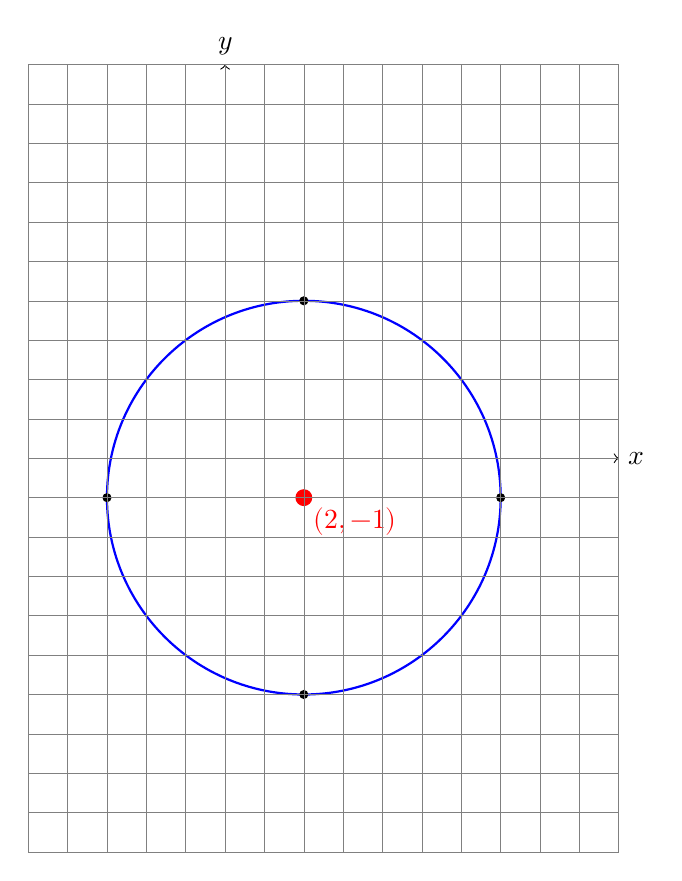
\begin{tikzpicture}[scale=0.5]
    % Draw axes
    \draw[->] (-5,0) -- (10,0) node[right] {$x$};
    \draw[->] (0,-10) -- (0,10) node[above] {$y$};
    
    % Draw the circle
    \draw[blue, thick] (2,-1) circle [radius=5];
    
    % Mark the center
    \filldraw[red] (2,-1) circle (0.2) node[below right] {$(2,-1)$};
    
    % Optional: mark radius points
    \filldraw[black] (2+5,-1) circle (0.1) node[below right] {};
    \filldraw[black] (2-5,-1) circle (0.1) node[below left] {};
    \filldraw[black] (2,-1+5) circle (0.1) node[above left] {};
    \filldraw[black] (2,-1-5) circle (0.1) node[below left] {};
    
    % Optional: grid
    \draw[very thin, gray] (-5,-10) grid[step=1] (10,10);
\end{tikzpicture}

\subsection{The Ellipse}

\begin{tcolorbox}[title=Problem 1, breakable]
    Sketch the graph of the following equations.
    In each case, indicate the center of the ellipse,
    and its extremities.
    \[\frac{x^2}{16} + \frac{y^2}{4} = 1\]
\end{tcolorbox}

\textbf{Solution:} Center is $(0, 0)$.
Extremities are $(\pm 4, 0)$ and $(0, \pm 2)$.
\begin{figure}[h!]
    \centering
    \includegraphics[width=0.5\textwidth]{images/ellipse_again.png}
\end{figure}

\subsection{The Hyperbola}

\begin{tcolorbox}[title=Problem 8, breakable]
    Sketch the graphs of the following curves, defined by the 
    given equations.

    $xy = 4$.
\end{tcolorbox}

\begin{figure}[h!]
    \centering
    \includegraphics[width=0.5\textwidth]{images/hyperbola.png}
\end{figure}

\subsection{Rotation of Hyperbolas}

\begin{tcolorbox}[title=Problem 2, breakable]
    Rotate the hyperbola $H$ defined by the equation $xy = 1$
    by $-\pi/4$. What is the equation satisfied by the image of $H$.
\end{tcolorbox}
\[v^2 - u^2 = 2\]

\begin{tcolorbox}[title=Problem 8, breakable]
    Prove the statement made in the text: If $G$ is rotation 
        and $F_r$ is a dilation by $r$, $G \circ F = F \circ G$.
\end{tcolorbox}

\begin{proof}
    Let $P = (x, y)$ be an arbitrary point.
    A dilation by $r$ is
    \[
    F_r(P) = r \begin{bmatrix} x \\ y \end{bmatrix},
    \]
    and a rotation by angle $\theta$ is 
    \[
    G(P) = \begin{bmatrix} \cos\theta & -\sin\theta \\ \sin\theta & \cos\theta \end{bmatrix} \begin{bmatrix} x \\ y \end{bmatrix}.
    \]
    Then
    \[
    G(F_r(P)) 
    = \begin{bmatrix} \cos\theta & -\sin\theta \\ \sin\theta & \cos\theta \end{bmatrix} \left( r \begin{bmatrix} x \\ y \end{bmatrix} \right)
    = r \begin{bmatrix} \cos\theta & -\sin\theta \\ \sin\theta & \cos\theta \end{bmatrix} \begin{bmatrix} x \\ y \end{bmatrix}.
    \]
    Similarly,
    \[
    F_r(G(P)) 
    = r \left( \begin{bmatrix} \cos\theta & -\sin\theta \\ \sin\theta & \cos\theta \end{bmatrix} \begin{bmatrix} x \\ y \end{bmatrix} \right)
    = r \begin{bmatrix} \cos\theta & -\sin\theta \\ \sin\theta & \cos\theta \end{bmatrix} \begin{bmatrix} x \\ y \end{bmatrix}.
    \]
\end{proof}
% Week 7: Connect derivatives to geometric interpretation. Practice tangent lines and normals.

\section{Increasing/Decreasing and Mean Value Theorem}
\subsection{Definition of a Function}

\begin{tcolorbox}[title=Problem 2, breakable]
    For what numbers could you define a function $f$
    by the formula
    \[f(x) = \frac{1}{x^2 - 2}\]
    What is the value of the function for $x = 5$.
\end{tcolorbox}

\textbf{Solution:}
$f$ is defined at all real numbers other than $\pm \sqrt{2}$.
\[f(5) = \frac{1}{5^2 - 2} = \frac{1}{23}\]

\begin{tcolorbox}[title=Problem 8, breakable]
    A function (defined for all numbers) is said to be 
    an \textbf{even} function if
    $f(x) = f(-x)$ for all numbers $x$. It is said to be 
    an \textbf{odd} function if $f(x) = -(f(-x))$ for all $x$.
    Determine which of the following functions are even or odd.

    (a) $f(x) = x$

    (b) $f(x) = x^2$

    (c) $f(x) = x^3$

    (d) $f(x) = \frac{1}{x} \text{ if } x \ne 0 \text{ and } f(0)=0$
\end{tcolorbox}

\textbf{Solution (a):} odd

\textbf{Solution (b):} even

\textbf{Solution (c):} odd

\textbf{Solution (d):} odd

\begin{tcolorbox}[title=Problem 9, breakable]
    Show that any function defined for all numbers 
    can be written as a sum of an even and an odd function.
    [Hint: The term 
    \[\frac{f(x) + f(-x)}{2}\]
    will be an even function.]
\end{tcolorbox}

\begin{proof}
    Let any function $f$ be defined for all numbers.
    \[
    g(x) = \frac{f(x) + f(-x)}{2}, \quad
    l(x) = \frac{f(x) - f(-x)}{2}.
    \]
    Then $g$ is even and $l$ is odd, and
    \[
    f(x) = g(x) + l(x).
    \]
\end{proof}

\begin{tcolorbox}[title=Problem 11, breakable]
    (a) Show that the sum of odd functions is odd.

    (b) Show that the sum of even functions is even.
\end{tcolorbox}

\begin{proof}
    Let $f, g$ be odd functions. Then
    \[
    (f + g)(x) = f(x) + g(x) = -f(-x) - g(-x) = -(f(-x) + g(-x)) = -(f + g)(-x),
    \]
    so the sum is odd.
    Let $f, g$ be even functions. Then
    \[
    (f + g)(x) = f(x) + g(x) = f(-x) + g(-x) = (f + g)(-x),
    \]
    so the sum is even.
\end{proof}

\begin{tcolorbox}[title=Problem 12, breakable]
    Determine whether the product of the following types of functions 
    is odd, even, or neither. Prove your assertions.

    (a) Product of odd function with odd function 

    (b) Product of even function with odd function 

    (c) Product of even function with even function
\end{tcolorbox}

\begin{proof} 
    If $f$ and $g$ are odd:
    \[
    (fg)(-x) = f(-x)g(-x) = (-f(x))(-g(x)) = f(x)g(x) = (fg)(x)
    \]
    The product is even.
    
    If $f$ is even and $g$ is odd:
    \[
    (fg)(-x) = f(-x)g(-x) = f(x)(-g(x)) = -f(x)g(x) = -(fg)(x)
    \]
    The product is odd.

    If $f$ and $g$ are even:
    \[
    (fg)(-x) = f(-x)g(-x) = f(x)g(x) = (fg)(x)
    \]
    The product is even.
\end{proof}

\subsection{Polynomial Functions}

\begin{tcolorbox}[title=Problem 1, breakable]
\end{tcolorbox}

\begin{tcolorbox}[title=Problem 3, breakable]
\end{tcolorbox}

\begin{tcolorbox}[title=Problem 4, breakable]
\end{tcolorbox}

\subsection{Graphs of Functions}

\begin{tcolorbox}[title=Problem 1, breakable]
\end{tcolorbox}

\subsection{Exponential Function}

\begin{tcolorbox}[title=Problem 7, breakable]
\end{tcolorbox}

\subsection{Logarithms}

\begin{tcolorbox}[title=Problem 3, breakable]
\end{tcolorbox}

\begin{tcolorbox}[title=Problem 6, breakable]
\end{tcolorbox}
% Week 8: Focus on identifying intervals of increase/decrease, concavity, and applying MVT.

\section{Maximum and Minimum Values}
\subsection{Definition}

\begin{tcolorbox}[title=Problem 1, breakable]
    A particle starts from the point $(0, 6)$ in the plant.
    It is attracted by a magnet below the x-axis, and repelled 
    by a magnet along the y-axis in such a way that its coordinates 
        are given as a function of $t$ by 
    \[x(t) = 2t, y(t) = 6 - 15t^3\]
    (a) Find the time at which it hits the x-axis.

    (b) Give a simple equation in terms of $x$ and $y$ such that the coordinates $(x(t), y(t))$ of the particle 
        satisfy this equation. Sketch the graph of this equation.

    (c) Find the distance of the point at which the particle hits the x-axis from teh origin.

    (d) Find the time at which the particle is at distance $2$ units from the x-axis, below the x-axis.

    (e) Find the time at which the particle is at distance $5$ units from the x-axis, below the x-axis.

    (f) Find the time at which the particle is at distance $7$ units from the x-axis, below the x-axis.
\end{tcolorbox}

\textbf{Solution (a):}
We required $0 = 6 - 15t^3$. Thus $t = \sqrt[3]{\frac{6}{15}}$.

\textbf{Solution (b):}
\[y = 6 - 15\left(\frac{x}{3}\right)^3\]
\begin{figure}[h!]
    \centering
    \includegraphics[width=0.5\textwidth]{images/particle.PNG}
\end{figure}

\textbf{Solution (c):}
The distance is $\sqrt{(3 \cdot \sqrt[3]{\frac{6}{15}})^2}$ units.

\textbf{Solution (d):}
We require $-2 = 6 - 15t^3$. Thus $t = \sqrt[3]{\frac{8}{15}}$

\textbf{Solution (e):}
We require $-5 = 6 - 15t^3$. Thus $t = \sqrt[3]{\frac{11}{15}}$

\textbf{Solution (f):}
We require $-7 = 6 - 15t^3$. Thus $t = \sqrt[3]{\frac{13}{15}}$

\subsection{Formalism of Mappings}

\begin{tcolorbox}[title=Problem 1, breakable]
    Let $f : S \longrightarrow T$ and $g : S \longrightarrow T$ be mappings. 
    Let 
    \[h = T \longrightarrow U\]
    be a mapping have an inverse mapping denoted by
    \[h^{-1} : U \longrightarrow T\]
    If 
    \[h \circ f = h \circ g\]
    Prove that $f = g$. This is the \textbf{cancellation law} for mappings.
\end{tcolorbox}

\begin{proof}
    Composing with $h^{-1}$ shows $f = g$.
\end{proof}

\begin{tcolorbox}[title=Problem 2, breakable]
    Let $f : S \longrightarrow T$ be a mapping having an inverse mapping.
    Prove the following statements.

    (a) If $x, y$ are elements of $S$ and $f(x) = f(y)$, then $x = y$.

    (c) If $z$ is an element of $T$, then there exists an element $x$ of $S$ such that $f(x) = z$.
\end{tcolorbox}

\begin{proof}
    Suppose $x, y$ are elements of $S$, and $f(x) = f(y)$. Composing with $f^{-1}$ shows $x = y$.
\end{proof}

\begin{proof}
    Suppose $z$ is an element of $T$.
    There exists $c \in S$ such that $f^{-1}(z) = c$. Composing with $f$ shows 
        $f(c) = z$.
\end{proof}

\subsection{Permutations}

\begin{tcolorbox}[title=Problem 10, breakable]
    Prove that the number of odd permutations of $J_n$
    for $n \ge 2$ is equal to the number of even permutations.
\end{tcolorbox}

\begin{proof}
    Let $\sigma_1, \ldots, \sigma_m$ be all the distinct even permutations.
    Let $\gamma$ be a transposition.
    Suppose $\sigma_i = \gamma_1 \gamma_2 \ldots \gamma_{2k}$
        for some $k \in \mathbb{Z}$.
    Composing with $\gamma$ we see $\gamma \sigma_i = \gamma \gamma_1 \gamma_2 \ldots \gamma_{2k}$
        is a product of $2k + 1$ transpositions, thus an odd permuation.
    Suppose $i \ne j$, $\gamma \sigma_i = \gamma \sigma_j$.
    Composing with $\gamma$ shows $\sigma_i = \sigma_j$, which is a contradiction.
    Thus $\gamma \sigma_1, \ldots, \gamma \sigma_m$ are distinct.
    Now suppose there exists an odd permuation not generated through this process.
    Let $\pi$ be this permutation.
    Then, $\pi$ can be written as a product of $2k + 1$ transpositions.
    Thus $\gamma \pi$ is a product of $2k$ transpositions, thus an even permutation,
        which must be in out list $\sigma_1, \ldots, \sigma_m$.
    Thus $\pi$ is of the form $\gamma \sigma_i$ for some $i$,
        and no odd permutation is as required.
\end{proof}

\begin{tcolorbox}[title=Problem 11, breakable]
    Prove that the number of permuations of $J_n$ is equal to $n!$.
\end{tcolorbox}

\begin{proof}
    (\textbf{Base Case}) Let $n = 1$. There is $1$ way to permute $1$ element, thus $1 = 1!$ as required.

    (\textbf{Induction Step}) Suppose for some $n \in \mathbb{N}$
        the theorem holds.
    Thus there are $n!$ ways to permute $n$ elements.
    Consider a permuation of $n + 1$ elements.
    By the induction hypothesis there are $n!$ ways to permute the first $n$ elements.
    For each of these permutations, there are $n + 1$ positions to place the $(n + 1)$-th 
    element, including placing it in its original position.
    Thus we have a total of $n!(n + 1) = (n + 1)!$ permuations as required.
\end{proof}

% Week 9: Practice finding local and global extrema. Connect with derivative tests.

\section{Curve Sketching, Concavity, Symmetry}
\subsection{The Complex Plane}

\begin{tcolorbox}[title=Problem 3, breakable]
    Let $z$ be a complex number $\ne 0$. What is the absolute value of $z \sqrt{z}$?
\end{tcolorbox}

\textbf{Solution:} Let $z = x + yi$. 
\[
|z \sqrt{z}| = |z| \, |\sqrt{z}| = (x^2 + y^2)^{1/2} \cdot (x^2 + y^2)^{1/4} = (x^2 + y^2)^{3/4} = (z \overline{z})^{3/4} = (|z|^2)^{3/4} = |z|^{3/2}
\]

\begin{tcolorbox}[title=Problem 4, breakable]
    Prove the statements of Theorem $1$.
\end{tcolorbox}

\begin{enumerate}
    \item $\overline{zw} = \overline{z} \overline{w}$
    \item $\overline{z + w} = \overline{z} + \overline{w}$
    \item $\overline{\overline{z}} = z$
\end{enumerate}

\begin{proof}
    Let $z = x + yi$ and $w = u + vi$. Then
    \[
    zw = (x + yi)(u + vi) = (xu - yv) + (xv + yu)i, \quad \overline{zw} = (xu - yv) - (xv + yu)i
    \]
    and
    \[
    \overline{z} \, \overline{w} = (x - yi)(u - vi) = (xu - yv) - (xv + yu)i.
    \]
    Therefore $\overline{zw} = \overline{z} \, \overline{w}$.
    \[
    z + w = (x+u) + (y+v)i, \quad \overline{z + w} = (x+u) - (y+v)i = (x - yi) + (u - vi) = \overline{z} + \overline{w}.
    \]
    \[
    \overline{\overline{z}} = \overline{x - yi} = x + yi = z.
    \]
\end{proof}


\begin{tcolorbox}[title=Problem 5, breakable]
    Show that for any complex number $z = x + iy$, with $x, y$ real, we have 
    \[Im(z) \le |Im(z)| \le |z|\]
\end{tcolorbox}

\begin{proof}
    Notice
    \[
    \operatorname{Im}(z) = y.
    \]
    By definition of absolute value
    \[
    y \le |y| = |\operatorname{Im}(z)|.
    \]
    Then
    \[
    |\operatorname{Im}(z)| = |y| \le \sqrt{x^2 + y^2} = |z|.
    \]
    Combining these inequalities shows
    \[
    \operatorname{Im}(z) \le |\operatorname{Im}(z)| \le |z|.
    \]
\end{proof}

\subsection{Polar Form}

\begin{tcolorbox}[title=Problem 3, breakable]
    Let $z$ be a complex number $ \ne 0$.
    Show that there are precisely two distinct complex numbers 
        whose square is $z$.
\end{tcolorbox}

\begin{proof}
    We first show existence of two complex numbers whose square are $z$.
    Let $z = r e^{\theta i}$ where $\theta, r \in \mathbb{R}$
        and $0 \le \theta < 2 \pi$.
    Consider $\sqrt{r} e^{\theta/2 i}$. Notice 
    \[\sqrt{r} e^{\theta/2 i} \cdot \sqrt{r} e^{\theta/2 i} = r e^{\theta i}\]
    Now consider $-\sqrt{r} e^{\theta/2 i}$. Since $z \ne 0$, $\sqrt{r} \ne -\sqrt{r}$. Then 
    \[-\sqrt{r} e^{\theta/2 i} \cdot -\sqrt{r} e^{\theta/2 i} = r e^{\theta i}\]

    We now show these are the only two complex numbers whose square are $z$.
    Suppose $w$ is a complex number such that $w^2 = z = r e^{\theta i}$.
    Let $w = \rho e^{x i}$. Then
    \[
        w^2 = \rho^2 e^{2xi} = r e^{\theta i}
    \]
    Matching moduli shows $\rho = \sqrt{r}$.
    Matching arguments shows $2x = \theta + 2\pi k$ for some $k \in \mathbb{Z}$.
    Thus $x = \theta/2 + k\pi$.
    Since angles differing by $2\pi$ give the same complex number, only
    $k = 0, 1$ produce distinct values. These are exactly
    $\sqrt{r}e^{\theta i/2}$ and $-\sqrt{r}e^{\theta i/2}$.
\end{proof}

\begin{tcolorbox}[title=Problem 4, breakable]
    Let $z$ be a complex number $\ne 0$.
    Let $n$ be a positive integer.
    Show that there are $n$ distinct complex numbers $w$
        such that $w^n = z$.
    Write these complex numbers in polar form.
    The proof given that a polynomial of degree $\le n$
        has at most $n$ roots applies to the complex case,
        and thus we see that there are no other complex 
        numbers $w$ such that $w^n = z$ other than those 
        you have presumably written down.
\end{tcolorbox}

\begin{proof}
    We first show existence of $n$ complex numbers whose $n$-th power is $z$.  
    Let $z = r e^{\theta i}$ where $r, \theta \in \mathbb{R}$ and $0 \le \theta < 2\pi$.  
    Consider 
    \[
    w = r^{1/n} e^{(\theta + 2\pi k)i/n}, \quad k = 0, 1, \dots, n-1.
    \]  
    Notice that
    \[
    w^n = \bigl(r^{1/n} e^{(\theta + 2\pi k)i/n}\bigr)^n = r e^{\theta i} = z.
    \]  
    Since $k$ ranges from $0$ to $n-1$, these are $n$ distinct numbers.

    We now show that these are the only complex numbers whose $n$-th power is $z$.  
    Suppose $w$ is a complex number such that $w^n = z = r e^{\theta i}$.  
    Let $w = \rho e^{\phi i}$. Then
    \[
    w^n = \rho^n e^{n\phi i} = r e^{\theta i}.
    \]  
    Matching moduli gives $\rho = r^{1/n}$.  
    Matching arguments gives $n\phi = \theta + 2\pi k$ for some $k \in \mathbb{Z}$, so
    \[
    \phi = \frac{\theta + 2\pi k}{n}.
    \]  
    Angles differing by $2\pi$ give the same complex number, so only $k = 0, 1, \dots, n-1$ produce distinct values. These are exactly
    \[
    w = r^{1/n} e^{(\theta + 2\pi k)i/n}, \quad k = 0, 1, \dots, n-1.
    \]
\end{proof}

\begin{tcolorbox}[title=Problem 5, breakable]
    Write in polar form the $n$ complex numbers $w$ 
        such that $w^n = 1$. Plot all of these as points in the 
        plane $n = 2, 3, 4, 5$.
\end{tcolorbox}

\begin{center}
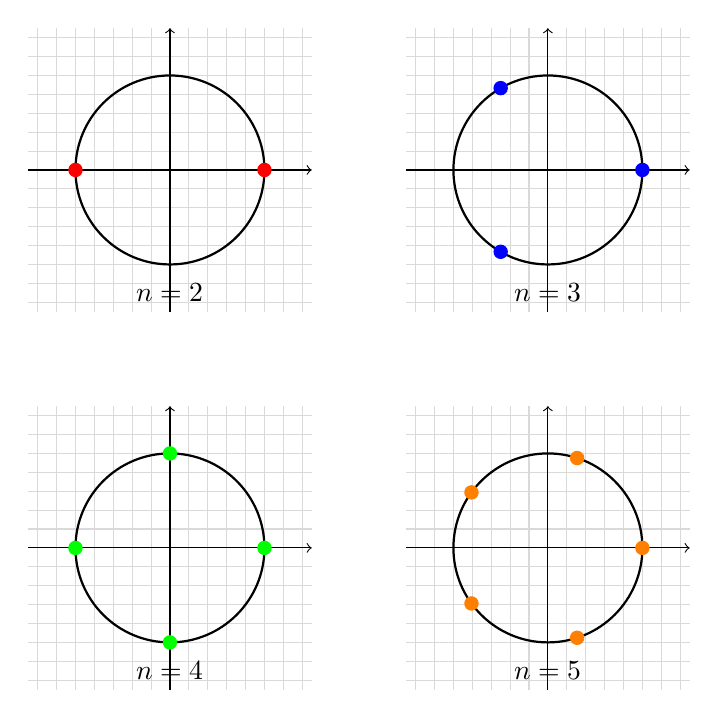
\begin{tikzpicture}[scale=1.2]
    % n = 2
    \begin{scope}[xshift=0cm, yshift=0cm]
    \draw[gray!30, step=0.2] (-1.5,-1.5) grid (1.5,1.5);
    \draw[->] (-1.5,0) -- (1.5,0);
    \draw[->] (0,-1.5) -- (0,1.5);
    \draw[thick] (0,0) circle(1);
    \foreach \k in {0,1} {
        \filldraw[red] ({cos(360*\k/2)}, {sin(360*\k/2)}) circle(2pt);
    }
    \node at (0,-1.3) {$n=2$};
    \end{scope}

    % n = 3
    \begin{scope}[xshift=4cm, yshift=0cm]
    \draw[gray!30, step=0.2] (-1.5,-1.5) grid (1.5,1.5);
    \draw[->] (-1.5,0) -- (1.5,0);
    \draw[->] (0,-1.5) -- (0,1.5);
    \draw[thick] (0,0) circle(1);
    \foreach \k in {0,1,2} {
        \filldraw[blue] ({cos(360*\k/3)}, {sin(360*\k/3)}) circle(2pt);
    }
    \node at (0,-1.3) {$n=3$};
    \end{scope}

    % n = 4
    \begin{scope}[xshift=0cm, yshift=-4cm]
    \draw[gray!30, step=0.2] (-1.5,-1.5) grid (1.5,1.5);
    \draw[->] (-1.5,0) -- (1.5,0);
    \draw[->] (0,-1.5) -- (0,1.5);
    \draw[thick] (0,0) circle(1);
    \foreach \k in {0,1,2,3} {
        \filldraw[green] ({cos(360*\k/4)}, {sin(360*\k/4)}) circle(2pt);
    }
    \node at (0,-1.3) {$n=4$};
    \end{scope}

    % n = 5
    \begin{scope}[xshift=4cm, yshift=-4cm]
    \draw[gray!30, step=0.2] (-1.5,-1.5) grid (1.5,1.5);
    \draw[->] (-1.5,0) -- (1.5,0);
    \draw[->] (0,-1.5) -- (0,1.5);
    \draw[thick] (0,0) circle(1);
    \foreach \k in {0,1,2,3,4} {
        \filldraw[orange] ({cos(360*\k/5)}, {sin(360*\k/5)}) circle(2pt);
    }
    \node at (0,-1.3) {$n=5$};
    \end{scope}
\end{tikzpicture}
\end{center}

\begin{tcolorbox}[title=Problem 6, breakable]
    If $\theta$ is real, show that 
    \[\cos \theta = \frac{e^{i \theta} + e^{-i \theta}}{2} \text{ and } \sin \theta = \frac{e^{i \theta} - e^{-i \theta}}{2i}\]
\end{tcolorbox}

\begin{proof}
    \begin{align*}
        \frac{e^{i \theta} + e^{-i \theta}}{2} 
            &= \frac{(\cos \theta + i \sin \theta) + (\cos(-\theta) + i \sin(-\theta))}{2} \\
            &= \frac{(\cos \theta + i \sin \theta) + (\cos \theta - i \sin \theta)}{2} \\
            &= \frac{2 \cos \theta}{2} \\
            &= \cos \theta
    \end{align*}
\end{proof}

\begin{proof}
    \begin{align*}
        \frac{e^{i \theta} - e^{-i \theta}}{2i} 
            &= \frac{(\cos \theta + i \sin \theta) - (\cos(-\theta) + i \sin(-\theta))}{2i} \\
            &= \frac{(\cos \theta + i \sin \theta) - (\cos \theta - i \sin \theta)}{2i} \\
            &= \frac{2 i \sin \theta}{2i} \\
            &= \sin \theta
    \end{align*}
\end{proof}
% Week 10: Combine derivative info to sketch curves. Focus on interpreting concavity and inflection points.

\section{Differentiation of Trigonometric Functions}
\subsection{Matrices}


In each of the following cases, write down the second row 
and first column of the indicated matrix.
Also write down its transpose.

\begin{tcolorbox}[title=Problem 1, breakable]
    \[\begin{bmatrix}
        2 & -5 \\
        -3 & -7
    \end{bmatrix}\]
\end{tcolorbox}

\textbf{Solution:}
Second row:
\[(-3, -7)\] 
First column:
\[\begin{bmatrix}
    2 \\
    -3
\end{bmatrix}\]
Transpose:
\[\begin{bmatrix}
    2 & -3 \\
    -5 & -7
\end{bmatrix}\]

\begin{tcolorbox}[title=Problem 4, breakable]
    \[\begin{bmatrix}
        3 & 5 & 6 \\
        -1 & 2 & 3 \\
        7 & 3 & -2
    \end{bmatrix}\]
\end{tcolorbox}

\textbf{Solution:}
Second row:
\[(-1, 2, 3)\] 
First column:
\[\begin{bmatrix}
    3 \\
    -1 \\
    7
\end{bmatrix}\]
Transpose:
\[\begin{bmatrix}
    3 & -1 & 7 \\
    5 & 2 & 3 \\
    6 & 3 & -2
\end{bmatrix}\]

\begin{tcolorbox}[title=Problem 7, breakable]
    Find the sum of the first two columns in the matrix in Exercise $4$.
\end{tcolorbox}

\textbf{Solution:}
\[\begin{bmatrix}
    3 \\
    5 \\
    6
\end{bmatrix} + \begin{bmatrix}
    -1 \\
    2 \\
    3
\end{bmatrix} = \begin{bmatrix}
    2 \\
    7 \\
    9
\end{bmatrix}\]

\subsection{Determinants of Order $2$}

\begin{tcolorbox}[title=Problem 2, breakable]
    Compute the determinant of 
    \[\begin{bmatrix}
        \cos \theta & -\sin \theta \\
        \sin \theta & \cos \theta
    \end{bmatrix}\]
\end{tcolorbox}

\textbf{Solution:}
\[D\left(\begin{bmatrix}
    \cos \theta & -\sin \theta \\
    \sin \theta & \cos \theta
\end{bmatrix}\right) = \cos \theta \cos \theta - (-\sin \theta)\sin \theta = \cos^2 \theta + \sin^2 \theta = 1\]

\begin{tcolorbox}[title=Problem 3, breakable]
    Compute the determinant 
    \[\begin{bmatrix}
        \cos \theta & \sin \theta \\
        \sin \theta & \cos \theta 
    \end{bmatrix}\]
    (a) $\theta = \pi$,

    (b) $\theta  = \pi/2$

    (c) $\theta = \pi/3$

    (d) $\theta = \pi/4$
\end{tcolorbox}

\textbf{General solution:}
\[D\left(\begin{bmatrix}
        \cos \theta & \sin \theta \\
        \sin \theta & \cos \theta 
\end{bmatrix}\right) = \cos \theta \cos \theta - \sin \theta \sin \theta = cos^2 \theta - sin^2 \theta\]

\textbf{Solution (a):} $cos^2 \pi - sin^2 \pi$

\textbf{Solution (b):} $cos^2 \pi/2 - sin^2 \pi/2$

\textbf{Solution (c):} $cos^2 \pi/3 - sin^2 \pi/3$

\textbf{Solution (d):} $cos^2 \pi/4 - sin^2 \pi/4$

\subsection{Properties of $2 \times 2$ Determinants}

\begin{tcolorbox}[title=Problem 1, breakable]
    Prove the other half of \textbf{D1}, i.e.
    distributivity on the other side other than that given in the text.
\end{tcolorbox}

\begin{proof}
    
    \begin{align*}
        D(C, B' + B'') &= D\left(\begin{bmatrix}
            b'_1 + b''_1 & c_1 \\
            b'_2 + b''_2 & c_2
        \end{bmatrix}\right) \\
                             &= c_2(b'_1 + b''_1) - c_1(b'_2 + b''_2) \\
                             &= c_2 b'_1 + c_2 b'_1 - c_1 b'_2 - c_1 b''_2 \\
                             &= D(C, B') + D(C, B'')
    \end{align*}
\end{proof}

\begin{tcolorbox}[title=Problem 2, breakable]
    Prove the other half of \textbf{D2}.
\end{tcolorbox}

\begin{proof}
    We have 
    \[D(B, xC) = D\left(\begin{bmatrix}
        b_1 & x c_1 \\
        b_2 & x c_2
    \end{bmatrix}\right) = x b_1 c_2 - x b_2 c_1 = x(b_1 c_2 - b_2 c_1) = x D(B, C)\]
\end{proof}

\begin{tcolorbox}[title=Problem 3, breakable]
    Prove the other half of \textbf{D5}.
\end{tcolorbox}

\begin{proof}
    Using \textbf{D1, D2, D4} we find 
    \[D(B, C + xB) = D(B, C) + D(B, xB) = D(B, C) + xD(B, B) = D(B, C)\]
\end{proof}

\begin{tcolorbox}[title=Problem 4, breakable]
    Using the same method as at the end of the section,
        find the value for $y$.
\end{tcolorbox}

\begin{proof}
    Suppose $x, y$ are solutions to the system of equations.
    We have 
    \[D(C, A) = D(xA + yB, A) = D(xA, A) + D(yB, A) = xD(A, A) + yD(B, A) = yD(B, A)\]
    Thus $y = \frac{D(C, A)}{D(B, A)}$.
\end{proof}

\begin{tcolorbox}[title=Problem 6, breakable]
    Let $c$ be a number, and let $A$ be a $2 \times 2$ matrix.
    Define $cA$ to be the matrix obtained by multiplying all components
    of $A$ by $c$. How does $D(cA)$ differ from $D(A)$.
\end{tcolorbox}

\textbf{Solution:} By \textbf{D2} it scales the value of the determinant by $c^2$.

\subsection{Determinants of Order $3$}

\begin{tcolorbox}[title=Problem 2 (a), breakable]
    Compute the following determinants by expandingaccording to the 
    second row, and also according to the third column.

    (a) \[\begin{bmatrix}
        3 & 1 & 2 \\
        0 & 3 & -1 \\
        4 & 1 & 1
    \end{bmatrix}\]
\end{tcolorbox}

\textbf{Solution:} By second row 
\[3(3 - 8) - (-1)(3 - 4) = -15 - 1 = -16\]
By third column 
\[2(0 - 12) - (-1)(3 - 4) + 1(9 - 0) = -24 - 1 + 9 = -16\]

\begin{tcolorbox}[title=Problem 4, breakable]
    Let $a, b, c$ be numbers. In terms of $a, b, c$
        what is the value of the determinant.
    \[\begin{bmatrix}
        a & 0 & 0 \\
        0 & b & 0 \\
        0 & 0 & c
    \end{bmatrix}\]
\end{tcolorbox}

\textbf{Solution:}
\[a(bc) = abc\]

\begin{tcolorbox}[title=Problem 6, breakable]
    In terms of the components of the matrix,  what is the value 
        of the determinant:
    \[(a) \begin{bmatrix}
        a_11 & a_12 & a_13 \\
        0 & a_22 & a_23 \\
        0 & 0 & a_33
    \end{bmatrix}, (b) \begin{bmatrix}
        a_11 & 0 & 0 \\
        a_21 & a_22 & 0 \\
        a_31 & a_32 & a_33
    \end{bmatrix}\]
\end{tcolorbox}

\textbf{Solution (a):}
\[a_{11}(a_{22} a_{33}) = a_{11} a_{22} a_{33}\]
\textbf{Solution (b):}
\[a_{11} a_{22} a_{33}\]

\subsection{Properties of $3 \times 3$ Determinants}

\begin{tcolorbox}[title=Problem 1, breakable]
    Write out in full and prove property \textbf{D1}
    with respect to the second and third column.
\end{tcolorbox}

\begin{theorem}
    Suppose that the second column can be written as a sum,
    \[A^2 = B + C\]
    that is,
    \[\begin{bmatrix}
        a_12 \\
        a_22 \\
        a_32
    \end{bmatrix} = \begin{bmatrix}
        b_1 \\
        b_2 \\
        b_3
    \end{bmatrix} + \begin{bmatrix}
        c_1 \\
        c_2 \\
        c_3
    \end{bmatrix}\]
    Then 
    \[D(A^1, B + C, A^3) = D(A^1, B, A^3) + D(A^1, C, A^3)\]
\end{theorem}

\begin{proof}
    We use the definition of the determinant, namely the expansion
    according to the second column. Each term splits into a sum of two
    terms corresponding to $B$ and $C$. For instance,
    \[a_{21} \begin{bmatrix}
        a_{12} & a_{13} \\
        a_{32} & a_{33} 
    \end{bmatrix} = b_1 \begin{bmatrix}
        a_{12} & a_{13} \\
        a_{32} & a_{33}
    \end{bmatrix} + c_1 \begin{bmatrix}
        a_{12} & a_{13} \\
        a_{32} & a_{33}
    \end{bmatrix}\]
    \[a_{22} \begin{bmatrix}
        b_2 + c_2 & a_{13} \\
        b_3 + c_3 & a_{33} 
    \end{bmatrix} = a_{22} \begin{bmatrix}
        b_2 & a_{13} \\
        b_3 & a_{33}
    \end{bmatrix} + a_{22} \begin{bmatrix}
        c_2 & a_{13} \\
        c_3 & a_{33}
    \end{bmatrix}\]
    \[a_{23} \begin{bmatrix}
        b_2 + c_2 & a_{12} \\
        b_3 + c_3 & a_{32} 
    \end{bmatrix} = a_{23} \begin{bmatrix}
        b_2 & a_{12} \\
        b_3 & a_{32}
    \end{bmatrix} + a_{23} \begin{bmatrix}
        c_2 & a_{12} \\
        c_3 & a_{32}
    \end{bmatrix}\]
    Summing with the appropriate signs yields the desired relation.
\end{proof}

\begin{theorem}
    Suppose that the third column can be written as a sum,
    \[A^3 = B + C\]
    that is,
    \[\begin{bmatrix}
        a_13 \\
        a_23 \\
        a_33
    \end{bmatrix} = \begin{bmatrix}
        b_1 \\
        b_2 \\
        b_3
    \end{bmatrix} + \begin{bmatrix}
        c_1 \\
        c_2 \\
        c_3
    \end{bmatrix}\]
    Then 
    \[D(A^1, A^2, B + C) = D(A^1, A^2, B) + D(A^1, A^2, C)\]
\end{theorem}

\begin{proof}
    We use the definition of the determinant, namely the expansion
    according to the third column. Each term splits into a sum of two
    terms corresponding to $B$ and $C$. For instance,
    \[a_{31} \begin{bmatrix}
        a_{12} & a_{13} \\
        a_{22} & a_{23} 
    \end{bmatrix} = b_1 \begin{bmatrix}
        a_{12} & a_{13} \\
        a_{22} & a_{23}
    \end{bmatrix} + c_1 \begin{bmatrix}
        a_{12} & a_{13} \\
        a_{22} & a_{23}
    \end{bmatrix}\]
    \[a_{32} \begin{bmatrix}
        b_2 + c_2 & a_{13} \\
        b_3 + c_3 & a_{23} 
    \end{bmatrix} = a_{32} \begin{bmatrix}
        b_2 & a_{13} \\
        b_3 & a_{23}
    \end{bmatrix} + a_{32} \begin{bmatrix}
        c_2 & a_{13} \\
        c_3 & a_{23}
    \end{bmatrix}\]
    \[a_{33} \begin{bmatrix}
        b_2 + c_2 & a_{12} \\
        b_3 + c_3 & a_{22} 
    \end{bmatrix} = a_{33} \begin{bmatrix}
        b_2 & a_{12} \\
        b_3 & a_{22}
    \end{bmatrix} + a_{33} \begin{bmatrix}
        c_2 & a_{12} \\
        c_3 & a_{22}
    \end{bmatrix}\]
    Summing with the appropriate signs yields the desired relation.
\end{proof}

\begin{tcolorbox}[title=Problem 2, breakable]
    Same thing for property \textbf{D2}.
\end{tcolorbox}

\begin{theorem}
    If $x$ is a number, then 
    \[D(A^1, x A^2, A^3) = x \cdot D(A^1, A^2, A^3)\]
\end{theorem}

\begin{proof}
We have:
\[
D(A^1, x A^2, A^3) =
- a_{11} \begin{vmatrix} x a_{22} & a_{23} \\ x a_{32} & a_{33} \end{vmatrix}
+ a_{21} \begin{vmatrix} x a_{12} & a_{13} \\ x a_{32} & a_{33} \end{vmatrix}
- a_{31} \begin{vmatrix} x a_{12} & a_{13} \\ x a_{22} & a_{23} \end{vmatrix}
= x \cdot D(A^1, A^2, A^3).
\]
\end{proof}

\begin{theorem}
    If $x$ is a number, then 
    \[D(A^1, A^2, x A^3) = x \cdot D(A^1, A^2, A^3)\]
\end{theorem}

\begin{proof}
We have:
\[
D(A^1, A^2, x A^3) =
a_{11} \begin{vmatrix} a_{22} & x a_{23} \\ a_{32} & x a_{33} \end{vmatrix}
- a_{21} \begin{vmatrix} a_{12} & x a_{13} \\ a_{32} & x a_{33} \end{vmatrix}
+ a_{31} \begin{vmatrix} a_{12} & x a_{13} \\ a_{22} & x a_{23} \end{vmatrix}
= x \cdot D(A^1, A^2, A^3).
\]
\end{proof}

\begin{tcolorbox}[title=Problem 3, breakable]
    Prove the two cases not treated in the text for 
    property \textbf{D4}.
\end{tcolorbox}

\begin{proof}
Suppose that $A_2 = A_3$, and look at the expansion of the determinant according to the first row. 
Then $a_{13} = a_{12}$, and the first two terms cancel. The third term is equal to 0 because it involves a 
$2 \times 2$ determinant whose two columns are equal. 
\end{proof}

\begin{proof}
Suppose that $A_1 = A_3$, and look at the expansion of the determinant according to the first row. 
Then $a_{13} = a_{11}$, and the first two terms cancel. The third term is equal to 0 because it involves 
a $2 \times 2$ determinant whose two columns are equal. 
\end{proof}

\begin{tcolorbox}[title=Problem 4, breakable]
Prove \textbf{D5}

(a) you add a multiple of the third column to the first;

(b) you add a multiple of the second column to the first;

(c) you add a third column to the second.
\end{tcolorbox}

\begin{proof}
    We have
    \[
        D(A_1 + x A_3, A_2, A_3) = D(A_1, A_2, A_3) + D(x A_3, A_2, A_3) \text{ (by D1)}
    \]
    \[
        = D(A_1, A_2, A_3) + x \cdot D(A_3, A_2, A_3) \text{ (by D2)}
        = D(A_1, A_2, A_3) \text{ (by D4).}
    \]
    We have
    \[
        D(A_1 + x A_2, A_2, A_3) = D(A_1, A_2, A_3) + D(x A_2, A_2, A_3) \text{ (by D1)}
    \]
    \[
        = D(A_1, A_2, A_3) + x \cdot D(A_2, A_2, A_3) \text{ (by D2)}
        = D(A_1, A_2, A_3) \text{ (by D4).}
    \]
    We have
    \[
        D(A_1, A_2 + A_3, A_3) = D(A_1, A_2, A_3) + D(A_1, A_3, A_3) \text{ (by D1)}
        = D(A_1, A_2, A_3) \text{ (by D4).}
    \]
\end{proof}

\begin{tcolorbox}[title=Problem 5, breakable]
    Prove \textbf{D6} in the second case.
\end{tcolorbox}

\begin{proof}
    \[
    0 = D(A_1, A_2 + A_3, A_2 + A_3)
    = D(A_1, A_2, A_2 + A_3) + D(A_1, A_3, A_2 + A_3)
    \]  
    \[
    = D(A_1, A_2, A_2) + D(A_1, A_2, A_3) + D(A_1, A_3, A_2) + D(A_1, A_3, A_3)
    = D(A_1, A_2, A_3) + D(A_1, A_3, A_2)
    \]
    Thus $D(A_1, A_2, A_3) = -D(A_1, A_3, A_2)$.
\end{proof}

\begin{tcolorbox}[title=Problem 6, breakable]
    If you interchange the first and third columns 
    of the given matrix, how does its determinant change?
    What about interchanging the first and third row?
\end{tcolorbox}

\textbf{Solution:} The determinant changes by a sign.

\begin{tcolorbox}[title=Problem 7, breakable]
    State \textbf{D5} and \textbf{D6} for rows.
\end{tcolorbox}

\begin{theorem}[D5 for rows]
If we add a multiple of one row to another, 
then the value of the determinant does not change. In other words, let $x$ be a number. Then, for instance,
\[
D(R_1 + x R_2, R_2, R_3) = D(R_1, R_2, R_3),
\]
and similarly in all other cases.
\end{theorem}

\begin{theorem}[D6 for rows]
If two adjacent rows are interchanged, then the determinant changes by a sign. In other words, we have
\[
D(R_2, R_1, R_3) = -D(R_1, R_2, R_3),
\]
and similarly in the other cases.
\end{theorem}

\begin{tcolorbox}[title=Problem 9, breakable]
    Let $c$ be a number and multiply each componenet 
    $a_{ij}$ of a $3 \times 3$ matrix $A$ by $c$, thus 
    obtaining a new matrix which we denote by $cA$.
    How does $D(A)$ differ from $D(cA)$.
\end{tcolorbox}

\textbf{Solution:} The determinant is scaled by $c^3$.

\begin{tcolorbox}[title=Problem 10, breakable]
    Let $x_1, x_2, x_3$ be numbers. Show that 
    \[
    \begin{vmatrix}
    1 & x_1 & x_1^2 \\
    1 & x_2 & x_2^2 \\
    1 & x_3 & x_3^2
    \end{vmatrix} = (x_2 - x_1)(x_3 - x_2)(x_3 - x_1)
    \]
\end{tcolorbox}

\begin{proof}
    Then
    \[
    \begin{vmatrix}
    1 & x_1 & x_1^2 \\
    1 & x_2 & x_2^2 \\
    1 & x_3 & x_3^2
    \end{vmatrix}
    = 1 \cdot (x_2 x_3^2 - x_3 x_2^2) 
    - x_1 \cdot (1 \cdot x_3^2 - 1 \cdot x_2^2) 
    + x_1^2 \cdot (1 \cdot x_3 - 1 \cdot x_2)
    = (x_2 - x_1)(x_3 - x_2)(x_3 - x_1).
    \]
\end{proof}

\begin{tcolorbox}[title=Problem 13, breakable]
    State the analogous property to that of Exercise $12$
    with respect to the second column. Then with respect 
    to the third column.
\end{tcolorbox}

\textbf{Solution (a):}
Let 
\[
A^2 = \sum_{j=1}^{n} x_j C^j
\]
where $C^j$ are column vectors and $x_j$ are numbers. Then
\[
D(A^1, A^2, A^3, \dots, A^n) = \sum_{j=1}^{n} x_j D(A^1, C^j, A^3, \dots, A^n).
\]

\textbf{Solution (b):}
Let 
\[
A^3 = \sum_{j=1}^{n} x_j C^j
\]
where $C^j$ are column vectors and $x_j$ are numbers. Then
\[
D(A^1, A^2, A^3, \dots, A^n) = \sum_{j=1}^{n} x_j D(A^1, A^2, C^j, \dots, A^n).
\]

\subsection{Cramer's Rule}

\begin{tcolorbox}[title=Problem 1, breakable]
    Fill in the missing steps in the proof of Cramer's rule.
    Cf. Exercises $11$ and $12$ of the proceeding section.
\end{tcolorbox}

\begin{proof}
    \begin{align*}
        D(B, A^2, A^3) &= D(x_1 A^1 + x_2 A^2 + x_3 A^3, A^2, A^3) \\
        &= D(x_1 A^1 + x_2 A^2, A^2, A^3) + D(x_3 A^3, A^2, A^3) \\
        &= D(x_1 A^1, A^2, A^3) + D(x^2 A^2, A^2, A^3) + D(x_3 A^3, A^2, A^3) \\
        &= x_1 D(A^1, A^2, A^3) + x_2 D(A^2, A^2, A^3) + x_3 D(A^3, A^2, A^3) \\
        &= x_1 D(A^1, A^2, A^3)
    \end{align*}
    Thus $x_1 = \frac{D(B, A^2, A^3)}{D(A^1, A^2, A^3)}$.
\end{proof}

\begin{tcolorbox}[title=Problem 2, breakable]
    Write out in full the proof of Cramer's rule for $x_2$ and $x_3$.
    It is very similar to the proof for $x_1$ in the text.
\end{tcolorbox}

\begin{proof}
    \begin{align*}
        D(B, A^1, A^3) &= D(x_1 A^1 + x_2 A^2 + x_3 A^3, A^1, A^3) \\
        &= D(x_1 A^1, A^1, A^3) + D(x_2 A^2 + x_3 A^3, A^1, A^3) \\
        &= D(x_1 A^1, A^1, A^3) + D(x_2 A^2, A^1, A^3) + D(x_3 A^3, A^1, A^3) \\
        &= x_1 D(A^1, A^1, A^3) + x_2 D(A^2, A^1, A^3) + x_3 D(A^3, A^1, A^3) \\
        &= x_2 D(A^2, A^1, A^3)
    \end{align*}
    Thus $x_2 = \frac{D(B, A^1, A^3)}{D(A^2, A^1, A^3)}$.
\end{proof}

\begin{proof}
    \begin{align*}
        D(B, A^1, A^2) &= D(x_1 A^1 + x_2 A^2 + x_3 A^3, A^1, A^2) \\
        &= D(x_1 A^1 + x_2 A^2, A^1, A^2) + D(x_3 A^3, A^1, A^2) \\
        &= D(x_1 A^1, A^1, A^2) + D(x_2 A^2, A^1, A^2) + D(x_3 A^3, A^1, A^2) \\
        &= x_1 D(A^1, A^1, A^2) + x_2 D(A^2, A^1, A^2) + x_3 D(A^3, A^1, A^2) \\
        &= x_3 D(A^3, A^1, A^2)
    \end{align*}
    Thus $x_2 = \frac{D(B, A^1, A^2)}{D(A^3, A^1, A^2)}$.
\end{proof}

\begin{tcolorbox}[title=Problem 3, breakable]
    Let $A^1, A^2, A^3$ be columns of a $3 \times 3$ matrix $A$,
    and assume that there are numbers $x_1, x_2, x_3$
    not all $0$ such that 
    \[x_1 A^1 + x_2 A^2 + x_3 A^3 = 0\]
    Prove that $D(A) = 0$.
\end{tcolorbox}

\begin{proof}
    Suppose wlog that $x_1 \ne 0$. 
    Then
    \[
        A^1 = -\frac{x_2}{x_1} A^2 - \frac{x_3}{x_1} A^3
    \]
    Clearly, $A^1$ is a linear combination of $A^2$ and $A^3$, so
    $D(A) = 0$.
\end{proof}
% Week 11: Review derivatives of sin, cos, tan, etc. Practice chain rule with trig functions.

\section{Inverse Trigonometric Functions}
\input{sections/chapter18.tex}
% Week 12: Learn derivatives of arcsin, arccos, arctan, etc. Connect to implicit differentiation.

\section{Related Rates}
\input{sections/chapter20.tex}
% Week 13: Focus on translating word problems into derivative equations. Practice multiple real-world scenarios.

\section{Differentials and Newton's Method}
\input{sections/chapter21.tex}
% Week 14: Understand differentials, linear approximations, and Newton-Raphson root-finding.

\section{Antiderivatives}
\begin{tcolorbox}[title=Problem 1, breakable]
    Complete the analysis of the symmetries 
    of the square, which we begain in the text.
    Some will be rotations, and some will be flips.
    Determine the matrix and permutation representations
    for them, draw a table of correspondence, and compute 
    the group table for your symmetries.
\end{tcolorbox} 

\textbf{Group Table:}
\[
\begin{array}{c|cccccccc}
\circ 
& \iota & p & p^2 & p^3 & \varphi & p\varphi & \varphi p & \varphi p^2 \\ \hline
\iota 
& \iota & p & p^2 & p^3 & \varphi & p\varphi & \varphi p & \varphi p^2 \\
p 
& p & p^2 & p^3 & \iota & p\varphi & \varphi p^2 & \varphi & \varphi p \\
p^2 
& p^2 & p^3 & \iota & p & \varphi p & \varphi p^2 & p\varphi & \varphi \\
p^3 
& p^3 & \iota & p & p^2 & \varphi p^2 & \varphi & \varphi p & p\varphi \\
\varphi 
& \varphi & \varphi p & \varphi p^2 & p\varphi & \iota & p & p^2 & p^3 \\
p\varphi 
& p\varphi & \varphi p^2 & \varphi & \varphi p & p & p^2 & p^3 & \iota \\
\varphi p 
& \varphi p & p\varphi & \varphi p^2 & \varphi & p^2 & p^3 & \iota & p \\
\varphi p^2 
& \varphi p^2 & \varphi & p\varphi & \varphi p & p^3 & \iota & p & p^2
\end{array}
\]
\textbf{Permutations:}
\[\iota \longleftrightarrow \begin{bmatrix}
    1 & 2 & 3 & 4 \\
    1 & 2 & 3 & 4
\end{bmatrix}, p \longleftrightarrow \begin{bmatrix}
    1 & 2 & 3 & 4 \\
    4 & 1 & 2 & 3
\end{bmatrix}, p^2 \longleftrightarrow \begin{bmatrix}
    1 & 2 & 3 & 4 \\
    3 & 4 & 1 & 2
\end{bmatrix}, p^3 \longleftrightarrow \begin{bmatrix}
    1 & 2 & 3 & 4 \\
    2 & 3 & 4 & 1
\end{bmatrix}\]
\[\varphi \longleftrightarrow \begin{bmatrix}
    1 & 2 & 3 & 4 \\
    2 & 1 & 4 & 3
\end{bmatrix}, p \varphi \longleftrightarrow  \begin{bmatrix}
    1 & 2 & 3 & 4 \\
    3 & 2 & 1 & 4
\end{bmatrix}, \varphi p \longleftrightarrow \begin{bmatrix}
    1 & 2 & 3 & 4 \\
    1 & 4 & 3 & 2
\end{bmatrix}, \varphi p^2 \longleftrightarrow \begin{bmatrix}
    1 & 2 & 3 & 4 \\
    4 & 3 & 2 & 1
\end{bmatrix}\]
\textbf{Table of Correspondence:}
\[
\begin{array}{c|cccc}
 & 1 & 2 & 3 & 4 \\ \hline
\iota        & 1 & 2 & 3 & 4 \\
p            & 4 & 1 & 2 & 3 \\
p^2          & 3 & 4 & 1 & 2 \\
p^3          & 2 & 3 & 4 & 1 \\
\varphi      & 2 & 1 & 4 & 3 \\
p\varphi     & 3 & 2 & 1 & 4 \\
\varphi p    & 1 & 4 & 3 & 2 \\
\varphi p^2  & 4 & 3 & 2 & 1
\end{array}
\]
\textbf{Matrix Correspondence:}
\[
\iota \longleftrightarrow 
\begin{bmatrix} 1 & 0 \\ 0 & 1 \end{bmatrix}, 
p \longleftrightarrow 
\begin{bmatrix} 0 & -1 \\ 1 & 0 \end{bmatrix}, 
p^2 \longleftrightarrow 
\begin{bmatrix} -1 & 0 \\ 0 & -1 \end{bmatrix}, 
p^3 \longleftrightarrow 
\begin{bmatrix} 0 & 1 \\ -1 & 0 \end{bmatrix}
\]
\[
\varphi \longleftrightarrow 
\begin{bmatrix} 1 & 0 \\ 0 & -1 \end{bmatrix}, 
p\varphi \longleftrightarrow 
\begin{bmatrix} 0 & 1 \\ 1 & 0 \end{bmatrix}, 
\varphi p \longleftrightarrow 
\begin{bmatrix} 0 & -1 \\ -1 & 0 \end{bmatrix}, 
\varphi p^2 \longleftrightarrow 
\begin{bmatrix} -1 & 0 \\ 0 & 1 \end{bmatrix}
\]

\begin{tcolorbox}[title=Problem 3, breakable]
    Determine all symmetries of a non-square rectangle,
    and represent them with matrices and permutations.
    How many rotations, and how many are flips.
\end{tcolorbox} 

\begin{proof}
    We simply remove the square symmetries constructed from $1$ or $3$ rotations.
    Thus there are $4$ symmetries of a non-square rectangle.
\end{proof}

\begin{tcolorbox}[title=Problem 5, breakable]
    Show algebraically that the rotation transformation 
    preserves distance: Consider the points 
    $P_1(x_1, y_1)$ and $P_2(x_2, y_2)$.

    (a) What is the square of the distance between $P_1$
        and $P_2$.

    (b) Now rotate through the angle $\theta$, by multiplying 
        by the appropriate matrix, to obtain the points 
        $P_1'(x_1', y_1')$ and $P_2'(x_2', y_2')$.
        Compute the square of the distance of these points.
        Use trig identities to show that this is the same 
        as in part a.
\end{tcolorbox} 

\textbf{Solution (a):}
The square of the distance between $P_1$ and $P_2$ is  
    $(x_2 - x_1)^2 + (y_2 - y_1)^2$.

\textbf{Solution (b):}
Notice 
\[
    \begin{bmatrix}x_1 & y_1\end{bmatrix}
    \begin{bmatrix}
                   \cos \theta & -\sin \theta \\
                   \sin \theta & \cos \theta
    \end{bmatrix} = 
    \begin{bmatrix}
     x_1 \cos\theta + y_1 \sin\theta, &
    -x_1 \sin\theta + y_1 \cos\theta
    \end{bmatrix}
\]
\[
    \begin{bmatrix}x_2 & y_2\end{bmatrix}
    \begin{bmatrix}
                   \cos \theta & -\sin \theta \\
                   \sin \theta & \cos \theta
    \end{bmatrix} = 
    \begin{bmatrix}
     x_2 \cos\theta + y_2 \sin\theta, &
    -x_2 \sin\theta + y_2 \cos\theta
    \end{bmatrix}
\]
Thus 
\[P_1'(x_1', y_1') = P_1'(x_1 \cos\theta + y_1 \sin\theta, -x_1 \sin\theta + y_1 \cos\theta),\]
and 
\[P_2'(x_2', y_2') = P_2'(x_2 \cos\theta + y_2 \sin\theta, -x_2 \sin\theta + y_2 \cos\theta).\]
Then the square of the distance between these points is 
\[((x_2 \cos\theta + y_2 \sin\theta) - (x_1 \cos\theta + y_1 \sin\theta))^2 
    + ((-x_2 \sin\theta + y_2 \cos\theta) - (-x_1 \sin\theta + y_1 \cos\theta))^2.\]
Some basic algebra show this simplifies to $(x_2 - x_1)^2 + (y_2 - y_1)^2$.

\begin{tcolorbox}[title=Problem 6, breakable]
    Verify by mutliplying two matrices together that a 
    rotation through angle $\theta$, followed by a 
    rotation through angle $\varphi$, gives a rotation through 
    angle $\theta + \varphi$.
\end{tcolorbox} 

\textbf{Solution:}
\[
\begin{bmatrix}
\cos \theta & -\sin \theta \\
\sin \theta & \cos \theta
\end{bmatrix}
\begin{bmatrix}
\cos \phi & -\sin \phi \\
\sin \phi & \cos \phi
\end{bmatrix}
=
\begin{bmatrix}
\cos\theta \cos\phi + (-\sin\theta)(\sin\phi) & \cos\theta(-\sin\phi) + (-\sin\theta)\cos\phi \\
\sin\theta \cos\phi + \cos\theta \sin\phi & \sin\theta(-\sin\phi) + \cos\theta \cos\phi
\end{bmatrix}
\]

\[
=
\begin{bmatrix}
\cos\theta \cos\phi - \sin\theta \sin\phi & -\cos\theta \sin\phi - \sin\theta \cos\phi \\
\sin\theta \cos\phi + \cos\theta \sin\phi & -\sin\theta \sin\phi + \cos\theta \cos\phi
\end{bmatrix}
\]

\[
=
\begin{bmatrix}
\cos(\theta+\phi) & -\sin(\theta+\phi) \\
\sin(\theta+\phi) & \cos(\theta+\phi)
\end{bmatrix}
\]

\begin{tcolorbox}[title=Problem 7, breakable]
    How many symmetries can you find for the unit circle?
    Which rotations are possible?
    Which flips?
\end{tcolorbox} 

\textbf{Solution:} There are an infinite number of 
symmetries for both flips and rotations on the unit circle.

\begin{tcolorbox}[title=Problem 8, breakable]
    Find out how many elements there are in $D_n$,
    the group of symmetries of a regular $n$-sided 
    polygon.
\end{tcolorbox} 

\textbf{Solution:}
There are $n$ rotations including the identity.
For each of these rotations we can flip granting another $n$ symmetries.
Thus there are $2n$ total symmetries.

\begin{tcolorbox}[title=Problem 9, breakable]
    You can check that all of the matrices of the 
    symmetries of the equilateral triangle and the 
    square have the property that their determinants 
    are always $\pm 1$ (See Exercise 8.2 for a 
    definition of the determinant of a $2 \times 2$
    matrix.) In this exercise you will show thaSt if a 
    matrix preserves distance, then its determinant 
    must be $1$.

    (a) Suppose that $A \in M_2(\mathbb{R})$, and let 
        $det(A) = 0$. Show that mutliplication by $A$ 
        cannot preserve distance. Do this by showing that 
        multiplication by $A$ takes some point in the plane 
        to the origin and hence cannot preserve distance.

    (b) Suppose next that 
        \[\begin{bmatrix}
            a & b \\
            c & d
        \end{bmatrix} = A \in M_2(\mathbb{R}),\]
        but $det(A) \ne 0$. Suppose that multiplication 
        by $A$ does preserve distance, and consider 
        successively what happens to 
        \[\begin{bmatrix}
            1 \\ 0
        \end{bmatrix},
        \begin{bmatrix}
            0 \\ 1
        \end{bmatrix}, 
        \begin{bmatrix}
            d \\ -c
        \end{bmatrix},
        \begin{bmatrix}
            -b \\ a
        \end{bmatrix}\]
        You will be able to infer that $det(A) = \pm 1$.
\end{tcolorbox} 

\begin{proof}
    Let $A = \begin{bmatrix}a & b \\ c & d\end{bmatrix}$ be an arbitrary matrix in $M_2(\mathbb{R})$ 
    such that $\det(A) = 0$. Then $\det(A) = ad - bc = 0$, so $ad = bc$.
    Let $\begin{bmatrix}x & y\end{bmatrix}$ be a point with $x, y \in \mathbb{R}$.  
    Applying the transformation $A$ gives 
    \[
    \begin{bmatrix}x & y\end{bmatrix}\begin{bmatrix}a & b \\ c & d\end{bmatrix} =
    \begin{bmatrix}ax + by & cx + dy\end{bmatrix}.
    \]
    If $a = b = c = d = 0$, then all points are mapped to the origin.  
    Suppose w.l.o.g. that $a \ne 0$. From $ax + by = 0$, we get $x = -\frac{b}{a}y$.  
    Substituting into $cx + dy = 0$ gives 
    \[
    c\left(-\frac{b}{a}y\right) + dy = \left(d - \frac{bc}{a}\right)y = 0.
    \]
    Since $\det(A) = ad - bc = 0$, we have $d - \frac{bc}{a} = 0$.  
    Thus, any point on the line $x = -\frac{b}{a}y$ is mapped to the origin by $A$.
\end{proof}

\[
A \begin{bmatrix}1 \\ 0\end{bmatrix} = 
\begin{bmatrix}a & b \\ c & d\end{bmatrix} \begin{bmatrix}1 \\ 0\end{bmatrix} = 
\begin{bmatrix}a \\ c\end{bmatrix}, \quad
A \begin{bmatrix}0 \\ 1\end{bmatrix} = 
\begin{bmatrix}a & b \\ c & d\end{bmatrix} \begin{bmatrix}0 \\ 1\end{bmatrix} = 
\begin{bmatrix}b \\ d\end{bmatrix},
\]
From this it follows that $a^2 + c^2 = 1$ and $b^2 + d^2 = 1$.
\[
A \begin{bmatrix}d \\ -c\end{bmatrix} = 
\begin{bmatrix}a & b \\ c & d\end{bmatrix} \begin{bmatrix}d \\ -c\end{bmatrix} = 
\begin{bmatrix}ad - bc \\ cd - cd\end{bmatrix} = 
\begin{bmatrix}ad - bc \\ 0\end{bmatrix}, \quad
A \begin{bmatrix}-b \\ a\end{bmatrix} = 
\begin{bmatrix}a & b \\ c & d\end{bmatrix} \begin{bmatrix}-b \\ a\end{bmatrix} = 
\begin{bmatrix}-ab + ab \\ -bc + ad\end{bmatrix} = 
\begin{bmatrix}0 \\ ad - bc\end{bmatrix}.
\]
We see that $|det(A)| = |ad - bc| = 1$ if distance is to be preserved.

\begin{tcolorbox}[title=Problem 10, breakable]
    Our description of the symmetries of the equilateral 
    triangle can be elegantly rephrased using the 
    arithmetic of the complex numbers $\mathbb{C}$,
    described in Chapter $8$.

    (a) Argue that the three vertices of the triangle can be thought 
        of as numbers of the form $e^{i \alpha_i}$ in the 
        complex plane, for appropriate angles $\alpha_i$.

    (b) Show that you can represent the rotations of the triangle 
        in the symmetry group by complex mutliplication by a 
        number of the form $e^{i \theta}$, for an 
        appropriate choice of $\theta$.

    (c) What operation on the complex numbers performs the flip 
        $\phi$?
\end{tcolorbox} 

\textbf{Solution (a):}The three vertices can be represented as
\[
e^{i \alpha_1}, \quad e^{i \alpha_2}, \quad e^{i \alpha_3},
\]
where $\alpha_1 = 0$, $\alpha_2 = 2\pi/3$, and $\alpha_3 = 4\pi/3$.  
The modulus is $1$ because the vertices are on the unit circle.

\textbf{Solution (b):}
Rotations of the triangle correspond to multiplication by 
\[
e^{i \theta}, \quad \theta \in \{0, 2\pi/3, 4\pi/3\}.
\] 

\textbf{Solution (c):}
A flip across a line through the origin is represented by complex conjugation $e^{-i \alpha_i}$, 
possibly combined with multiplication by $e^{i \phi}$.
% Week 15: Review basic antiderivatives, power rule, and substitution.

\section{Definite Integral and Area Under a Curve}
\begin{tcolorbox}[title=Problem 1, breakable]
    Find all symmetries of a pyramid as draw below 
    (the base is a square, and the four sides are congruent).
\end{tcolorbox} 

\textbf{Solution:}
There are $4$ symmetries by rotating the base $3$ times plus the identity.

\begin{tcolorbox}[title=Problem 3, breakable]
    Consider the \emph{flatlanders}, who live in the plane 
    and consequently cannot conceive of motion in three dimensions.
    Formulate a definition for $\mathbb{R}^2$ for flatlanders,
    and then determine for them the group of symmetries 
    of the equilateral triangle and the square.
\end{tcolorbox} 

\textbf{Solution:}
A symmetry is a one-to-one onto function $\beta : \mathbb{R}^2 \longrightarrow \mathbb{R}^2$
    which preserves distances and does not reverse the direction of any basis vector.
There are $4$ symmetries of the square and $3$ symmetries of the equilateral triangle 
under this definition of symmetry in $\mathbb{R}^2$.

\begin{tcolorbox}[title=Problem 8, breakable]
    Consider a cube with a special down face: This face is 
    different, and consequently, a symmetry must leave it alone; the 
    face might be rotated, but must remain the down face.
    (You might imagine a circular dot in the center of this face.)
    How many symmetries of the unmarked cube are still symmetries 
    of this cube.
\end{tcolorbox} 

\textbf{Solution:} The four symmetries that rotate the base.
% Week 16: Connect Riemann sums to definite integrals. Practice area computations.

\section{Fundamental Theorem of Calculus}
\begin{tcolorbox}[title=Problem 5, breakable]
    In this problem we consider permutations of the set $\mathbb{R}$.

    (a) Let $S(\mathbb{R})$ denote the set of all real-valued functions 
    $f : \mathbb{R} \longrightarrow \mathbb{R}$, such that $f$ is 
    \emph{one-to-one} and \emph{onto}. Prove that $S(\mathbb{R})$ is 
    a group, where the operation is functional composition.

    (b) Now let $A(\mathbb{R})$ be the set of functions from 
    $S(\mathbb{R})$ that are also \textbf{order preserving}: By 
    this we mean that if $x < y$, then $f(x) < f(y)$. Prove that 
    $A(\mathbb{R})$ is a group under functional composition.
\end{tcolorbox} 

\begin{proof}
Let $f, g, h \in S(\mathbb{R})$.
Furthermore, let $\iota : \mathbb{R} \longrightarrow \mathbb{R}$ be a function
defined by $\iota(x) = x$.
Notice that $\iota \in S(\mathbb{R})$.

\begin{proof}
    Let $f, g \in A(\mathbb{R})$.
    We know that $f$ and $g$ are bijections and order preserving.
    Let $\iota : \mathbb{R} \to \mathbb{R}$ be defined by $\iota(x)=x$.

    (\textbf{Rule 1})
    Let $x,y \in \mathbb{R}$ such that $x < y$.
    Since $g$ is order preserving, $g(x) < g(y)$.
    Since $f$ is order preserving, $f(g(x)) < f(g(y))$.
    Thus $(f \circ g)(x) < (f \circ g)(y)$.
    It follows that $f \circ g \in A(\mathbb{R})$.

    (\textbf{Rule 2})
    Suppose $x<y$. Then $\iota(x)<\iota(y)$, so $\iota$ is order preserving.
    Thus $\iota \in A(\mathbb{R})$.

    (\textbf{Rule 3})
    Let $f \in A(\mathbb{R})$.
    Since $f$ is a bijection, it has an inverse $f^{-1}$.
    Let $x,y \in \mathbb{R}$ such that $x<y$.
    Then $f(x) < f(y)$, and applying $f^{-1}$ gives
    $f^{-1}(x) < f^{-1}(y)$.
    It follows that $f^{-1}$ is order preserving, and $f^{-1} \in A(\mathbb{R})$.
\end{proof}


(\textbf{Rule 1})
    Let $x$ be an arbitrary real number.
    Notice $
    ((f \circ g) \circ h)(x)
    = (f \circ g)(h(x))
    = f(g(h(x)))
    = f((g \circ h)(x))
    = (f \circ (g \circ h))(x)$.

    (\textbf{Rule 2})
    Notice that $f \circ \iota = \iota \circ f = f$.

    (\textbf{Rule 3})
    Since $f$ is a bijection, it has an inverse $f^{-1}$ such that
    $f \circ f^{-1} = f^{-1} \circ f = \iota$.
\end{proof}

\begin{tcolorbox}[title=Problem 7, breakable]
    Let $n$ be a positive integer and $\mathcal{C}$ be a circle.
    Now for $i = 0, 1, \ldots, n - 1$, let $p_i$ be the rotation of 
    $\mathcal{C}$ counterclockwise through the angle 
    $2 \pi i / n$ radians. Show that this set of rotations is a group 
    under the operation of composition. How many elements are in this group?
\end{tcolorbox} 

\begin{proof}
Let $i, j \in \{x \in \mathbb{Z} \mid 0 \le x \le n-1\}$.

(\textbf{Rule 1})
    Notice that
    \[
    p_i \circ p_j = p_{\, (i+j)\bmod n} = p_j \circ p_i.
    \]
    It follow that the set of closed under composition.

    (\textbf{Rule 2})
    Notice that
    \[
    p_i \circ p_{\, (n-i)\bmod n} = p_0.
    \]

    (\textbf{Rule 3})
    Since $p_0$ is rotation by angle $0$, it follows that
    \[
    p_i \circ p_0 = p_0 \circ p_i = p_i.
    \]
\end{proof}

\textbf{Solution:} There are $n$ elements in this group.

\begin{tcolorbox}[title=Problem 8, breakable]
    Let $G$ be a group with operation $\circ$.
    Suppose that $x \circ x = 1$, for all $x \in G$.
    Prove that $G$ is abelian.
\end{tcolorbox} 

\begin{proof}
    Let $x, y \in G$.
    Then $x \circ y = (x \circ y)^{-1} = y^{-1} \circ x^{-1} = y \circ x$ as required.
\end{proof}

\begin{tcolorbox}[title=Problem 10, breakable]
    Let $R$ be any ring, and suppose that $\phi, \psi \in Aut(R)$.
    Show that the composition of $\phi \psi \in Aut(R)$, by checking 
    that this function has the appropriate domain and range, is one-to-one,
    onto, and preserves addition and mutiplication. (This exercise 
    verfies that $Aut(R)$ is closed under functional composition; in 
    Example 24.18 we complete the verification that $Aut(R)$ is a group under this 
    operation.)
\end{tcolorbox} 

\begin{proof}
    Since $dom(\phi \psi) = dom(\psi) = R$, the domain of $\phi \psi$ is valid.  
    Now, since $ran(\psi) = R$ and $\phi$ is one-to-one and onto, the range of the composition $\phi \psi$ is $R$.  

    Let $x, y \in R$.  
    Then $\phi(\psi(x)) = \phi(\psi(y))$, and since $\phi$ is one-to-one, it follows that $\psi(x) = \psi(y)$.  
    Then, since $\psi$ is one-to-one, $x = y$; thus $\phi \psi$ is one-to-one.  

    Now let $x$ be an arbitrary element in $R$.  
    Since $\phi$ is onto, there exists $y \in R$ such that $\phi(y) = x$.  
    Since $y \in R$ and $\psi$ is onto, there exists $z \in R$ such that $\psi(z) = y$.  
    Then $\phi \psi(z) = x$; thus $\phi \psi$ is onto.  

    Therefore $\phi \psi : R \longrightarrow R$ is a one-to-one, onto function as required.  

    Now let $x, y$ be arbitrary elements in $R$.  
    Then $(\phi \psi)(x + y) = \phi(\psi(x + y)) = \phi(\psi(x) + \psi(y))$.  
    Similarly, $(\phi \psi)(xy) = \phi(\psi(x)\psi(y))$.  
    Thus $\phi \psi$ is closed under addition and multiplication.
\end{proof}

\begin{tcolorbox}[title=Problem 11, breakable]
    Prove that $Aut(\mathbb{Z})$ is a group with only 
    a single element.
\end{tcolorbox} 

\begin{proof}
    Since $\mathbb{Z}$ is a ring, by problem $10$, $\langle Aut(\mathbb{Z}), \circ \rangle$ is a group.
    Now clearly $\iota \in Aut(\mathbb{Z})$.
    Let $\psi$ be an arbitrary automorphism in $Aut(\mathbb{Z})$.
    Consider $\psi(1 \cdot 1) = \psi(1^2) = \psi(1)\psi(1)$.
    Thus $\psi(1)^2 = \psi(1)$, which in $\mathbb{Z}$ has two solutions: $0$ and $1$.
    Suppose $\psi(1) = 0$. 
    Then $\psi$ would map all integers to $0$, contradicting bijectivity.
    To see this, let $x$ be an arbitrary integer.
    Then $x = \underbrace{1 + 1 + \cdots + 1}_{x \text{ times}}$,
    and it follows that $
        \psi(x) = \underbrace{\psi(1) + \psi(1) + \cdots + \psi(1)}_{x \text{ times}} 
                  = \underbrace{0 + 0 + \cdots + 0}_{x \text{ times}} = 0$.
    It follows that $\psi(1) = 1$.
    Therefore $\psi(x) = x$ for all $x \in \mathbb{Z}$, so $\psi = \iota$.
\end{proof}

\begin{tcolorbox}[title=Problem 11, breakable]
    Show that $Aut(\mathbb{Q})$ is a group with only 
    a single element.
\end{tcolorbox} 

\begin{proof} 
    Since $\mathbb{Q}$ is a ring, by problem $10$, $\langle Aut(\mathbb{Q}), \circ \rangle$ is a group. 
    Now clearly $\iota \in Aut(\mathbb{Q})$. 
    Let $\psi$ be an arbitrary automorphism in $Aut(\mathbb{Q})$. 
    Consider $\mathbb{Z} \subset \mathbb{Q}$. By problem $10$, we know that for $a \in \mathbb{Z}$, $\psi(a) = a$. 
    Now let $b \in \mathbb{Q} - \{0\}$ and note that 
    $
    \psi(1) = \psi\Big(b \cdot \frac{1}{b}\Big) = \psi(b) \psi\Big(\frac{1}{b}\Big) = b \cdot x = 1
    $.
    It must be that $x = \frac{1}{b}$, thus $\psi\Big(\frac{1}{b}\Big) = \frac{1}{b}$. 
    Then let $x \in \mathbb{Q}$ be written as $\frac{a}{b}$ with $a \in \mathbb{Z}$ and $b \in \mathbb{Z} - \{0\}$. 
    It follows that $\frac{a}{b} = a \cdot \frac{1}{b}$ and 
    $
    \psi\Big(a \cdot \frac{1}{b}\Big) = \psi(a) \psi\Big(\frac{1}{b}\Big) = a \cdot \frac{1}{b} = \frac{a}{b}
    $.
    Thus $\psi = \iota$, as required. 
\end{proof}

\begin{tcolorbox}[title=Problem 13, breakable]
    In this problem you will sketch the proof that $Aut(\mathbb{R})$ is a group 
    with only a single element. You will use the fact that all 
    positive real numbers have exactly two square roots.

    (a) Let $a, b, \in \mathbb{R}$. Show that $a \ge b$ if and only if 
    $a - b = x^2$, for some $x \in \mathbb{R}$.

    (b) Use part a to show that if $\rho \in Aut(\mathbb{R})$, then $a \ge b$
    if and only if $\rho(a) \ge \rho(b)$.

    (c) Argue that any automorphism of $\mathbb{R}$ is fixed on the rational 
    numbers $\mathbb{Q}$ (See Exercise 12.)

    (d) You may assume that between any two real numbers is a rational number.
    Use this to prove that any automorphism of $\mathbb{R}$ is fixed on all 
    real numbers, so $Aut(\mathbb{R})$ has only a single element.
\end{tcolorbox} 

\begin{proof}
($\longrightarrow$) 
    Suppose $a \ge b$.
    It follows that $a - b \ge 0$.
    Thus since $a - b \in \mathbb{R}$,
    there exists $x \in \mathbb{R}$
    such that $x^2 = a - b$.

    ($\longleftarrow$)
    Suppose $a - b = x^2$, for some $x \in \mathbb{R}$.
    It follows that $x^2 \ge 0$ thus $a \ge b$.
\end{proof}

\begin{proof}
    ($\longrightarrow$)
    Suppose $\rho \in Aut(\mathbb{R})$.
    Furthermore, suppose $a \ge b$.
    Then $a + (-b) = x^2 \ge 0$.
    Thus $\rho(a + (-b)) = \rho(a) + \rho(-b) = \rho(x^2) \ge \rho(0) = 0$.
    Therefore $\rho(a) \ge \rho(b)$ as required.

    ($\longleftarrow$) Suppose $\rho(a) \ge \rho(b)$.
    Then $\rho(a) - \rho(b) \ge \rho(0) \iff \rho(a + (-b)) \ge \rho(0)$.
    Thus $a + (-b) \ge 0$ and it follows that $a \ge b$.
\end{proof}

\begin{proof}
    This follows directly from Problem 12 since $\mathbb{Q} \subset \mathbb{R}$.
\end{proof}

\begin{proof}
    Now, since the rationals are fixed, if $\rho$ is not the identity it 
        must be that an irrational number was mapped to a different irrational number.
    That is, for some $x \in \mathbb{R}$ such that $x$ is irrational,
        $\rho(x) = z$ such that $z$ is irrational and $x \ne z$.
    Consider some arbitrary rational number between $x$ and $z$, say $l$.
    Now there are two cases: either $x < l < z$ or $x > l > z$.
    Then, wlog suppose $x < l < z$.
    It follows that $\rho(x) < \rho(l) < \rho(z)$, but $\rho(l) = l$ and $\rho(x) = z$,
    thus $z < l < \rho(z)$, which is a contradiction.
    Thus the real numbers are fixed.
    It follows that $Aut(\mathbb{R})$ contains one element $\iota$.
\end{proof}

\begin{tcolorbox}[title=Problem 14, breakable]
    Consider the field of complex numbers $\mathbb{C}$, and its group of automorphisms
    $Aut(\mathbb{C})$. Show that this group has only two elements,
    namely the identity automorphism $\iota$, and the 
    complex conjugate map $\phi$ defined by $\phi(a + b) = a - bi$.
    (See Exercise 16.4).
\end{tcolorbox} 

\begin{proof}
    Clearly $\iota \in Aut(\mathbb{C})$.  
    Let $\rho \in Aut(\mathbb{C})$.  
    Then $\rho$ must fix all real numbers from Problem 13.  
    Now consider $\rho(i)$. Since $i^2 = -1$ it follows that $\rho(i)^2 = \rho(i^2) = \rho(-1) = -1$.  
    Thus $\rho(i) = i$ or $\rho(i) = -i$.  
    Therefore, for any $a + bi \in \mathbb{C}$, either $\rho(a + bi) = a + bi$ or $\rho(a + bi) = a - bi$.  
    Thus $Aut(\mathbb{C})$ has exactly two elements: $\iota$ and $\phi$.
\end{proof}



% Week 17: Understand both parts of the theorem and applications to evaluating integrals.

\section{Applications: Area and Arc Length}
\input{sections/chapter29.tex}
% Week 18: Solve area between curves and arc length problems.

\section{Applications: Volume}
\input{sections/chapter30.tex}
% Week 19: Focus on disk, washer, and shell methods. Practice multiple setup problems.

\section{Techniques of Integration I: Integration by Parts}
\input{sections/chapter31.tex}
% Week 20: Practice by parts on polynomial × trig/exponential functions.

\section{Techniques of Integration II: Trig Integrands / Trig Substitutions}
\input{sections/chapter32.tex}
% Week 21: Focus on trig integrals and substitutions. Recognize patterns quickly.

\section{Techniques of Integration III: Partial Fractions}
\input{sections/chapter33.tex}
% Week 22: Practice decomposing rational functions and integrating. Very common in Calc 3 review.

\section{Improper Integrals}
\input{sections/chapter35.tex}
% Week 23: Understand convergence/divergence and setup of improper integrals.

\section{Parametric Representation of Curves}
\input{sections/chapter37.tex}
% Week 24: Review derivatives of parametric equations and tangent lines.

\section{Plane Vectors}
\input{sections/chapter39.tex}
% Week 25: Intro to vectors in 2D. Useful for moving into 3D vectors in Calc 3.

\section{Polar Coordinates}
\input{sections/chapter41.tex}
% Week 26: Practice plotting, derivatives, and areas in polar coordinates.

\section{Sequences}
\input{sections/chapter42.tex}
% Week 27: Understand limits of sequences and convergence intuition.

\section{Series}
\input{sections/chapter43.tex}
% Week 28: Practice convergence tests (integral, comparison, ratio, alternating). Do multiple examples.

\section{Power Series}
\input{sections/chapter46.tex}
% Week 29: Focus on representing functions as series and finding interval of convergence.

\section{Taylor and Maclaurin Series}
\input{sections/chapter47.tex}
% Week 30: Practice expansions of common functions (e^x, sin x, cos x, ln(1+x)). Connect derivatives to series coefficients.

\end{document}
